\documentclass[review,3p,times,authoryear]{elsarticle}


\biboptions{round,authoryear}
\usepackage{setspace}
\onehalfspacing

\usepackage{booktabs}
\usepackage{amssymb}
\usepackage{amsmath}
\usepackage{subcaption}
\usepackage{amsthm}
\usepackage{algorithm}
\usepackage{algpseudocode}
\newtheorem{definition}{Definition}
\usepackage{float}
\usepackage{algpseudocode}
\usepackage{titlesec}
\usepackage{indentfirst}
\usepackage{threeparttable}
\usepackage{comment}
\usepackage{longtable}
\usepackage{array}

\newcounter{proposition}
\newcounter{lemma}

\newenvironment{proposition}[1][]{%
	\refstepcounter{proposition}%
	\par\medskip
	\noindent\textbf{Proposition~\arabic{proposition}.} \itshape
}{%
	\par\medskip
}

\newenvironment{lemma}[1][]{%
	\refstepcounter{lemma}%
	\par\medskip
	\noindent\textbf{Lemma~\arabic{lemma}.} \itshape
}{%
	\par\medskip
}


\titleformat{\paragraph}
  {\normalfont\normalsize\bfseries}
  {\theparagraph}{1em}{}

\titlespacing*{\paragraph}
  {0pt}{1ex}{0.5ex}

\setlength{\parindent}{2em}

\usepackage{multirow}
\usepackage{graphicx}
\renewcommand{\topfraction}{0.9}
\renewcommand{\bottomfraction}{0.9}
\renewcommand{\textfraction}{0.05}
\renewcommand{\floatpagefraction}{0.9}
\usepackage[
    colorlinks=true, 
    linkcolor=blue, 
    citecolor=blue, 
    urlcolor=blue,
    pdftitle={Optimizing batch formation policies for the cost--lead time trade-offs in additive manufacturing production systems}
]{hyperref}

\usepackage{booktabs}

\usepackage{chngcntr}


\begin{document}

\begin{frontmatter}

\title{Exact Scheduling of Parallel Additive Manufacturing Machines for Total Tardiness Minimization}





\begin{abstract}
	This paper studies the one-dimensional batch scheduling problem for parallel
	additive manufacturing (AM) machines with the objective of minimizing total
	tardiness. We develop a tailored exact branch-and-bound algorithm that branches
	on the assignment of parts to machines and evaluates each complete assignment by
	decomposing it into independent single-machine subproblems. Each subproblem is
	solved exactly by a dedicated single-machine AM scheduling oracle that combines
	batch-position branching, valid parallel and positional lower bounds, and
	dominance pruning. At the parallel-machine level, a node lower bound is obtained
	by combining oracle-based bounds on the assigned parts with per-part tardiness
	floors on the free parts, and a memoization pool reuses oracle values to both
	avoid recomputation and strengthen the node bound. The incumbent upper bound is
	produced by a multi-rule constructive heuristic refined by a move-based local
	search. Computational experiments show that the algorithm proves optimality for
	instances with up to $17$ parts within seconds on the single machine, and that
	on the parallel-machine problem a corrected depth-first diving rule reduces both
	the search-tree size and the peak memory by up to several orders of magnitude
	relative to a balance-first rule, while leaving the proven optimum unchanged. We further report a negative
	result: a parallel positional free-part bound is structurally dominated by the
	per-part floor and yields no additional pruning.
\end{abstract}

\begin{keyword}
Additive manufacturing \sep Parallel machine scheduling \sep Batch scheduling \sep Total tardiness \sep Branch-and-bound \sep Exact algorithm
\end{keyword}

\end{frontmatter}

%%%%%%%%%%%%%%%%%%%%%%%%%%%%%%%%%%%%%%%%%%%%%%%%%%%%%%%%%%%%%%%%%%%%%%%%%%%%%%%%

\section{Introduction}
Metal additive manufacturing has been increasingly adopted not only in established sectors such as aerospace, automotive, and healthcare, but also in emerging applications including robotics and unmanned aerial vehicles. Representative examples include customized stainless-steel robotic grippers fabricated by laser powder bed fusion and topology-optimized Ti-6Al-4V frames developed for unmanned aerial vehicles.

To meet the growing demand for customized metal parts, manufacturers commonly operate multiple AM machines in parallel. As illustrated in Fig. 1, heterogeneous parts with different geometries, dimensions, build heights, and due dates must be assigned to machines, grouped into feasible build batches, and sequenced for processing. Parts grouped into the same batch are fabricated simultaneously on a common build platform and therefore share the completion time of that batch. Once a batch is completed, its constituent parts become available for delivery, and their completion times directly affect whether individual due dates can be met.


\begin{figure*}[!t]
	\centering
	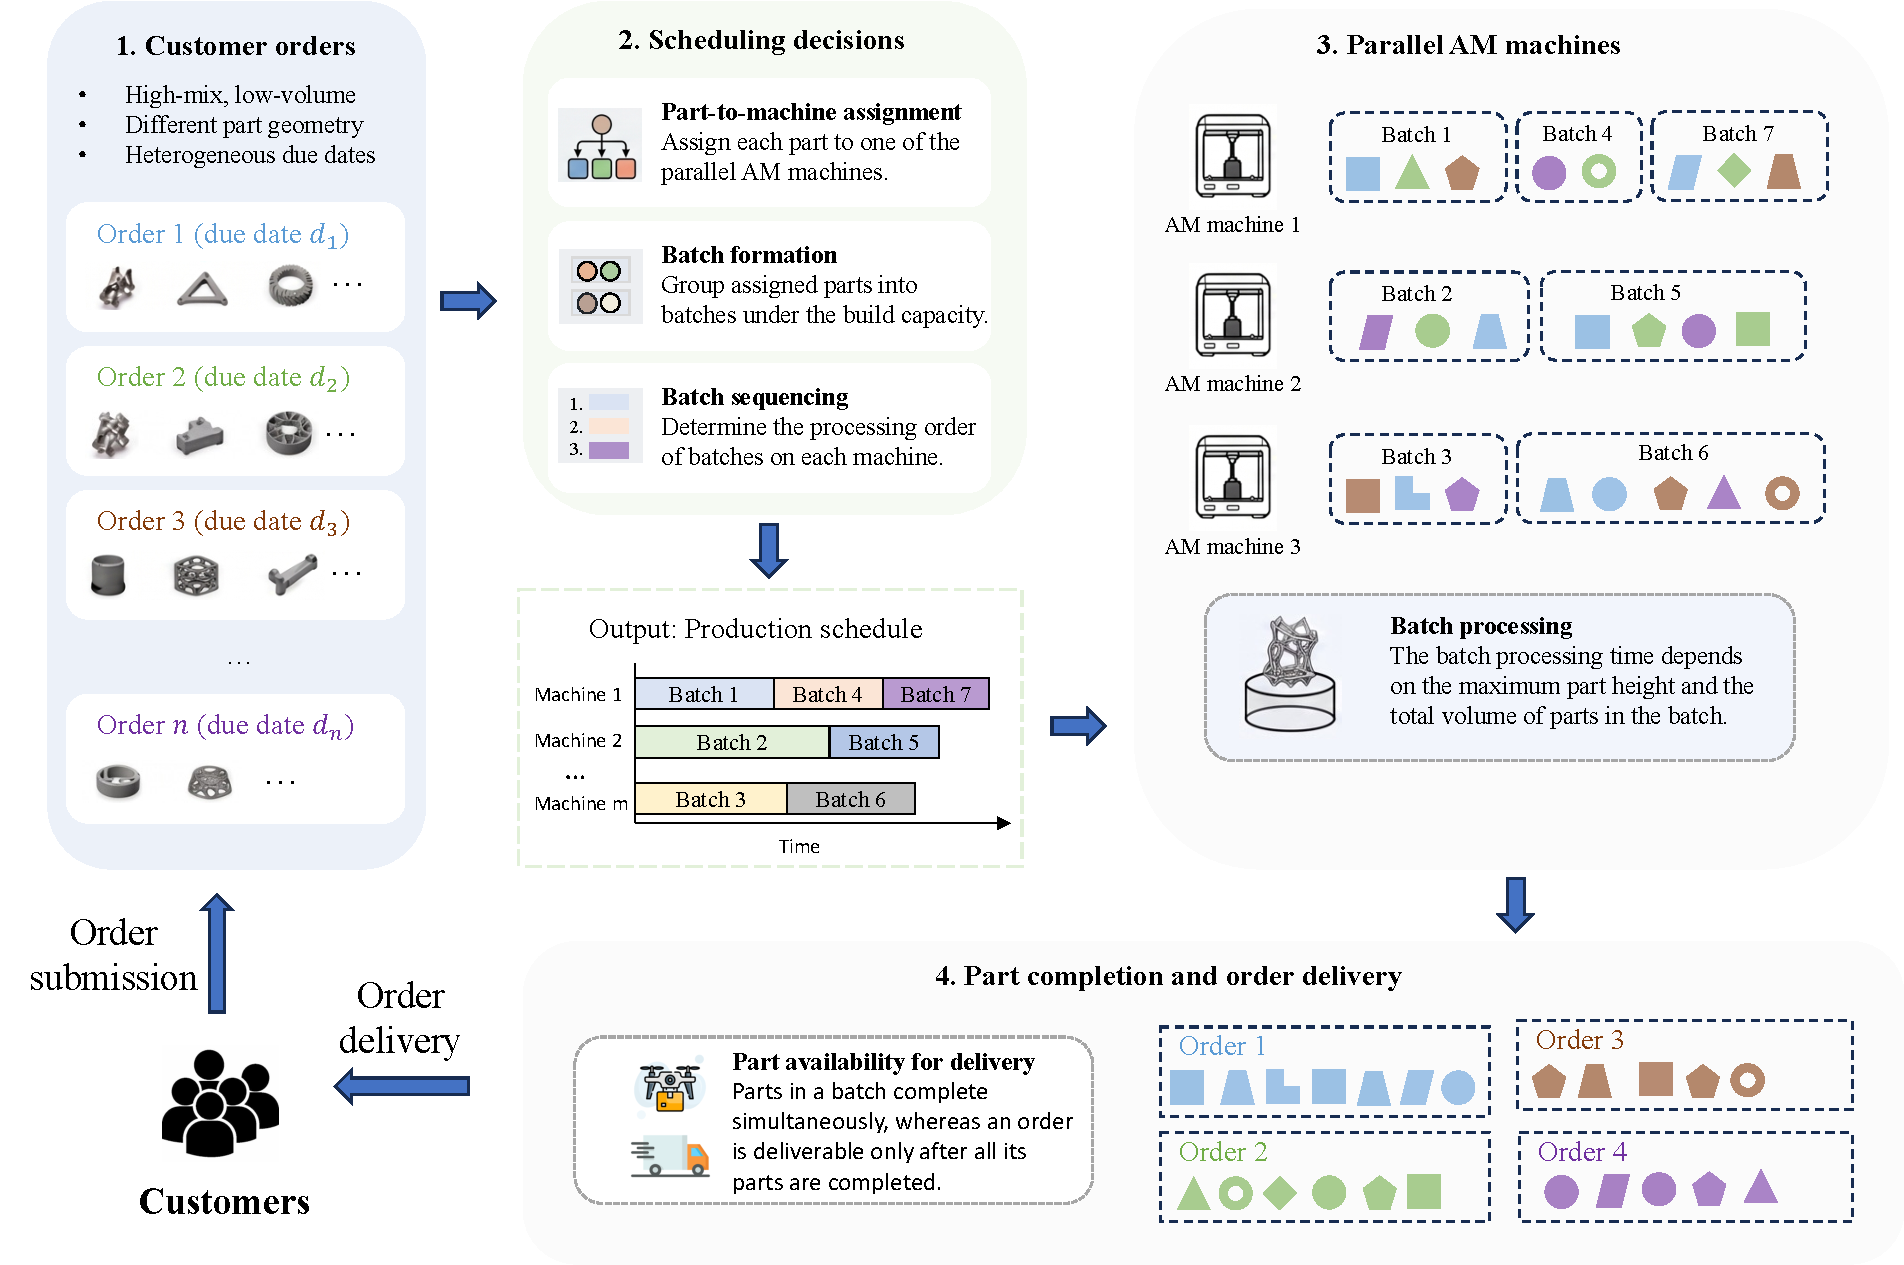
\includegraphics[width=\textwidth]{Figures/Cloud AM Scheduling.pdf}
	\caption{Illustration of the scheduling process in a parallel metal additive manufacturing system, including customer orders, part-to-machine assignment, batch formation, batch sequencing, batch processing, and order delivery.}
	\label{fig:cloud_am_scheduling}
\end{figure*}


Machine assignment, batch formation, and batch sequencing directly determine part completion times and therefore have a substantial impact on due-date performance. Ineffective scheduling decisions may result in considerable total tardiness, making scheduling a critical operational problem in parallel metal AM systems. Accordingly, a growing body of research has investigated production scheduling problems in AM systems.

Most of the AM scheduling studies focus on makespan optimizatiion, only a few takcles the due-date performance. Yu et al. 2022 study the scheduling of unrelated parallel AM machines for total tardiness. Wu et al. 2022 consider the scheduling problem of a cloud AM system. Wu eet al. 2025 studies the scheduling problem of unrelated parallel AM machines to reduce tardy delivery, while considering the uncertainties in processing times. However, these studies relay on heuristic or metaheuristics that cannot provide guarantees on optimality. 

Exact approaches for AM scheduling have been receiving increasing attentions. Zipfel et al. (2024) propose a branch and cut method for makespan optimization of parallel AM machines. Mao et al. (2024) propose a combinatorial benders decomposition appraoch for the same problem. To the best of our knowledge, Nascimento et al. 2024 is the only study that tackles the total tardiness for parallel AM machines. They use the combinatorial bedners decompostion framework, where the master problem is a 1D simplified batch machine scheduling problem, and the subproblem checkes the bin-packing feasibility of unregular 2D parts. Nascimento et al. 2026 further improves the efficiency of the framework by XXX. However, in these studies, the p-batch assumption is made for the batch processing time, i.e., the batch processing time equal to the longest processing time of the part in the batch. While in metal additive manufacturing, this might not be accurate. 

\begin{figure}[tb]
	\begin{center}
		\centering
		\resizebox*{15.0cm}{!}{
\includegraphics{figures/SLM Process.pdf}}\hspace{1pt}
		\caption{The process of SLM. In the powder material layering stage, the build platform is lowered by a specific amount corresponding to the thickness of the next layer. Then, a recoater blade moves a thin layer of powder from the powder container to the printing area. After, in the laser melting stage, the laser scans the specified area, melting the powder to form a solid structural layer of the part. These steps continues untill the build is completed. }
		\label{fig:slm_process}
	\end{center}
\end{figure}

Fig. 2 shows the process of printing a batch with SLM technology. The batch processing time consists of mainly three parts: batch setup time (inlucidng preheating and cooling), recoating time (related to the highest part height in the batch), and the laser scanning time, which is proportional to the total volume of parts in the batch. This means that, as the number of parts in the batch grows, the batch processing time would increase obviously, which makes the batch a mix-batch rather than a p-batch. According to the real-world experiments performed by Lv et al. (2021), the laser scanning time can account for about 25 \% of the total batch processing time. This percentage can go up to 50\% when a fuller batch is used, as shown in Lin and Yu (2025). Neglecting such factor (i.e., use the longest )would generate considerable biase between the model and the real implemtation. 

Replacing the p-batch assumption by the more realistic m-batch feature is non-trival. Firstly, it makes the decision problem more complex because "packing as more as possible parts into a batch" is no longer a thumb of rule for the total tardiness objective because a full batch might lead to a long processing time and pospone the delivery for all parts in the batch. The scheduler has to balance between sharing common batch time and maintaining delivery flexibility, as indicated by Yu et al. (2022). Second, the chanllenge also comes from the computational perspective. According to our numerical experiments (detained in Section XX), replacing the batch time calculation in the MILP model for the parallel AM scheduling problem dramatically lower the sovability of the model in 3600 seconds. The underly reason is due to a looser lower bound of the LP relaxation of the original model. Such impact is large. Because currently most of the exact approach for nesting and scheduling on AM machines relay on the logit-base benders decomposition framework whose master problem is a scheduling problem with bin-packing relaxation, and typically soved by off-the-shelf solver such as Cplex or gurobi. When the master scheduling problem becomes hard to solve, the application of these methods becomes difficult. And an efficient ad-hoc approach to solve the master problem becomes importance, which we believe is not be proposed. 

Motivated by this gap, this study focus on the schedulng problem for parallel AM machines to mimize the total tardiness. We aim at proposing an efficent exact approach for solving the scheduling problem, where the nesting part is simplied by a 1D capacity constraint. Our contribution is as follows:





\section{LITERATURE REVIEW}

\subsection{Nesting and Scheduling in Additive Manufacturing}

Additive manufacturing (AM) enables the direct fabrication of customized parts
from digital models and is increasingly used in production environments where
small lot sizes, geometric flexibility, and short response times are important
\citep{attaranRise3DPrinting2017}. From an operations-planning perspective,
however, AM does not eliminate scheduling complexity. In powder-bed processes,
several parts may be produced simultaneously in the same build, so production
planning must decide not only which machine processes each part but also how
parts are grouped into builds, how they are nested on the build platform, and
in what sequence the resulting batches are processed.

Recent reviews emphasize that nesting and scheduling are tightly coupled in AM
systems \citep{ohNestingSchedulingProblems2020,
pintoNestingSchedulingOptimization2024}. The nesting decision determines the
feasibility and composition of each build, while the scheduling decision
determines the completion time of the parts assigned to that build. This
coupling distinguishes AM scheduling from classical single-job machine
scheduling. A batch may contain multiple parts with different due dates and
geometries, and all parts in the same batch share the same completion time.
Consequently, batch formation decisions directly influence customer-service
objectives such as tardiness.

\subsection{Optimization Models for AM Scheduling}

The AM scheduling literature has studied several operational settings and
objective functions. Early mixed-integer programming models focused mainly on
makespan minimization and demonstrated that even simplified AM machine
scheduling problems can be computationally challenging
\citep{kucukkocMILPModelsMinimise2019}. Subsequent work incorporated richer AM
features, such as orientation selection and two-dimensional packing
\citep{cheMachineSchedulingOrientation2021}, total tardiness on parallel AM
machines \citep{yuMathematicalModelsMinimizing2022}, uncertain processing times
on parallel machines \citep{wuNestingSchedulingParallel2025}, and energy-aware
nesting and scheduling on selective laser melting machines
\citep{yuMathematicalProgrammingModel2024}. These studies show that AM
scheduling models must often combine machine assignment, batching, sequencing,
and geometry-dependent processing times.

The present study is closest to the stream that considers customer-oriented
objectives on parallel AM machines. In total-tardiness settings, the objective
depends on individual part completion times rather than only on the final
makespan. This feature changes the role of batching: grouping parts can improve
capacity utilization, but it can also delay urgent parts if they wait for a
later or longer batch. This trade-off is especially important under realistic
AM processing-time structures where the processing time of a batch depends on
both the total volume of the parts and the maximum part height.

\subsection{Exact Algorithms for AM Nesting and Scheduling}

Because AM nesting and scheduling problems combine packing and sequencing
decisions, exact algorithms have received increasing attention. Several recent
studies use decomposition to separate the combinatorial nesting decisions from
the scheduling or sequencing decisions. \citet{nascimentoOptimalDecompositionApproach2024}
propose an optimal decomposition approach for large AM nesting and scheduling
problems, and \citet{nascimentoImprovingEfficiencyLogicbased2026} further
improve logic-based Benders decomposition for p-batch scheduling problems with
two-dimensional packing. \citet{maoCombinatorialBendersDecomposition2024}
develop a combinatorial Benders decomposition for a single-machine AM
scheduling problem with two-dimensional packing constraints. Related exact
methods include branch-and-cut approaches for integrated AM planning
\citep{zipfelNewBranchandcutApproach2024}, nested Benders decompositions for
order acceptance and AM scheduling
\citep{chenBendersDecompositionsOrder2026}, and logic-based Benders
decomposition for AM scheduling on unrelated parallel machines
\citep{chenLogicBasedBenders2026}.

These exact methods provide important algorithmic ideas, but they do not
directly solve the problem considered in this paper. Some focus on
single-machine AM scheduling, while others address makespan, order acceptance,
or p-batch processing assumptions. In p-batch models, the processing time of a
batch is typically governed by the longest or largest job in the batch. By
contrast, in powder-bed AM the laser scanning component is additive in the
volumes of all parts in the batch, whereas the recoating component depends on
the maximum height. This mixed processing-time structure makes adding a part to
a batch beneficial for reducing the number of setups but costly because it
increases the volume-dependent processing time and delays subsequent batches.

\subsection{Exact Algorithms for Parallel-Machine Scheduling}

The upper-level structure of our problem is also related to the exact
parallel-machine scheduling literature. Classical exact methods include
assignment-based branch-and-bound algorithms, cutting-plane approaches, and
set-partitioning or column-generation formulations. For example,
\citet{mokotoffExactAlgorithmIdentical2004} propose an exact algorithm for
identical parallel-machine scheduling, while \citet{chenSolvingParallelMachine1999}
solve parallel-machine scheduling problems by column generation. Branch-and-price
and branch-price-and-cut methods have also become central tools for difficult
parallel-machine scheduling variants, because they can represent complete
single-machine schedules as columns and provide strong lower bounds.

However, the AM setting changes the computational role of the single-machine
subproblem. In many classical parallel-machine models, once the jobs assigned
to a machine are fixed, evaluating or optimizing the single-machine schedule is
comparatively straightforward or can be handled by a well-structured pricing
routine. In the AM batch scheduling problem studied here, the single-machine
subproblem remains NP-hard because it must jointly determine feasible batch
compositions and their sequence. A branch-and-price formulation would therefore
require solving a hard AM batch-scheduling pricing problem repeatedly. This
observation motivates the nested exact framework developed in this paper:
the upper-level search branches on part-to-machine assignments, while each
complete assignment is evaluated by a dedicated exact single-machine oracle
whose results are memoized and reused across the search tree.

\subsection{Research Gap and Positioning of This Study}

The above literature suggests three gaps. First, existing AM exact algorithms
have made substantial progress on nesting and scheduling, but most are designed
for single-machine settings, p-batch assumptions, makespan-oriented objectives,
or decomposition structures different from the total-tardiness problem studied
here. Second, AM studies that explicitly consider parallel machines and total
tardiness are still limited in exact algorithmic development, and direct MILP
formulations become difficult even for moderate instance sizes. Third,
classical exact algorithms for parallel-machine scheduling provide useful
branching and decomposition principles, but they cannot be applied directly
because the machine-level AM batching subproblem is itself a difficult exact
scheduling problem.

This paper addresses these gaps by studying the identical parallel-machine
one-dimensional AM batch scheduling problem with the objective of minimizing
total tardiness. The proposed exact algorithm combines an assignment-based
parallel-machine branch-and-bound search with an exact single-machine AM
scheduling oracle. The oracle handles the AM-specific batching and sequencing
decisions, while the upper-level search exploits symmetry reduction,
oracle-based lower bounds, memoization, and heuristic upper bounds to prove
optimality for small and medium-sized instances.

\section{MATHEMATICAL PROGRAMMING MODEL}

\subsection{Problem Description}
A set of parts $J=\{1,\dots,n\}$ is to be processed on a set of identical
parallel metal additive manufacturing machines $M=\{1,\dots,\bar M\}$
based on Powder Bed Fusion technology. Without loss of generality, we assume
that each customer order consists of a single part, so that order tardiness
is equivalent to part tardiness. Each part $j \in J$ has a due date $d_j$, a
volume $v_j$, and fixed geometric dimensions given by length $l_j$, width
$w_j$, and height $h_j$. All machines are assumed to have identical
rectangular build platforms, each with length $L$ and width $W$.

Parts are assigned to machines and grouped into batches. On each machine,
batches are processed sequentially from time zero, while different machines
can process their assigned batches in parallel. We consider a
one-dimensional capacity restriction, under which a set of parts can be
assigned to the same batch if the sum of their projected areas does not
exceed the platform capacity $L \times W$. This assumption gives rise to the
identical parallel-machine one-dimensional batch scheduling problem studied
in this paper.

The processing time of a batch consists of three components: the fixed
machine setup time $S$, the laser scanning time, and the recoating time
\cite{cheMachineSchedulingOrientation2021}. More specifically, the laser
scanning time depends on the total volume of the parts assigned to the
batch, whereas the recoating time depends on the maximum height of the parts
in the batch. Let $P_{mb}$ denote the processing time of batch position $b$
on machine $m$, and let $C_{mb}$ denote its completion time. If part $j$ is
assigned to batch position $b$ on machine $m$, then its completion time
$c_j$ is equal to $C_{mb}$. The tardiness of part $j$ is defined as
\[
T_j=\max\{0,\,c_j-d_j\}.
\]
All parts are assumed to be available at time zero. The objective is to
determine the assignment of parts to machines, the grouping of parts into
batches on each machine, and the sequence of batches on each machine so as
to minimize the total tardiness of all parts.

\subsection{MILP Formulation}
We formulate the identical parallel-machine one-dimensional batch scheduling problem as a mixed-integer linear program (MILP). The formulation extends the single-machine model by introducing machine-indexed batch positions. Each part must be assigned to exactly one batch on exactly one machine, and batches on the same machine are processed sequentially from time zero. Since the machines are identical, the processing-time structure of each batch remains the same across machines.

\noindent \textbf{Sets and Indices}
\begin{itemize}
	\item $J = \{1, \dots, n\}$: Set of parts.
	\item $M = \{1, \dots, \bar M\}$: Set of identical parallel machines.
	\item $B = \{1, \dots, n\}$: Set of available batch positions on each machine.
\end{itemize}

\noindent \textbf{Parameters}
\begin{itemize}
	\item $l_j, w_j, h_j$: Length, width, and height of part $j$.
	\item $v_j$: Volume of part $j$.
	\item $d_j$: Due date of part $j$.
	\item $L, W$: Length and width of the build platform.
	\item $S$: Setup time of a machine.
	\item $V$: Laser scanning time coefficient.
	\item $U$: Recoating time coefficient.
	\item $\mathcal{M}$: A sufficiently large positive constant.
\end{itemize}

\noindent \textbf{Decision Variables}
\begin{itemize}
	\item $x_{jmb}$: equal to 1 if part $j$ is assigned to batch position $b$ on machine $m$, 0 otherwise.
	\item $z_{mb}$: equal to 1 if batch position $b$ on machine $m$ is used, 0 otherwise.
	\item $H_{mb}$: height of batch $b$ on machine $m$.
	\item $P_{mb}$: processing time of batch $b$ on machine $m$.
	\item $C_{mb}$: completion time of batch $b$ on machine $m$.
	\item $c_j$: completion time of part $j$.
	\item $T_j$: tardiness of part $j$.
\end{itemize}

The MILP formulation is given as follows:
\begin{equation}
	\text{Minimize} \quad \sum_{j \in J} T_j
	\label{obj_pm}
\end{equation}

\noindent \textbf{s.t.}

\begin{flalign}
	& \sum_{m \in M} \sum_{b \in B} x_{jmb} = 1,
	\quad \forall j \in J
	& \label{eq:pm_assign} \\
	%
	& \sum_{j \in J} x_{jmb} \le \mathcal{M} z_{mb},
	\quad \forall m \in M,\ \forall b \in B
	& \label{eq:pm_link_xz} \\
	%
	& \sum_{j \in J} (l_j w_j)\, x_{jmb} \le LW,
	\quad \forall m \in M,\ \forall b \in B
	& \label{eq:pm_area} \\
	%
	& H_{mb} \ge h_j x_{jmb},
	\quad \forall j \in J,\ \forall m \in M,\ \forall b \in B
	& \label{eq:pm_height} \\
	%
	& P_{mb} = S z_{mb} + V \sum_{j \in J} v_j x_{jmb} + U H_{mb},
	\quad \forall m \in M,\ \forall b \in B
	& \label{eq:pm_proctime} \\
	%
	& C_{m1} \ge P_{m1},
	\quad \forall m \in M
	& \label{eq:pm_Cfirst} \\
	%
	& C_{mb} \ge C_{m,b-1} + P_{mb},
	\quad \forall m \in M,\ \forall b = 2,\dots,|B|
	& \label{eq:pm_Cseq} \\
	%
	& c_j \ge C_{mb} - \mathcal{M}(1-x_{jmb}),
	\quad \forall j \in J,\ \forall m \in M,\ \forall b \in B
	& \label{eq:pm_cj} \\
	%
	& T_j \ge c_j - d_j,
	\quad \forall j \in J
	& \label{eq:pm_tard1} \\
	%
	& T_j \ge 0,
	\quad \forall j \in J
	& \label{eq:pm_tard2} \\
	%
	& z_{m,b+1} \le z_{mb},
	\quad \forall m \in M,\ \forall b = 1,\dots,|B|-1
	& \label{eq:pm_sym1} \\
	%
	& x_{jmb}, z_{mb} \in \{0,1\},
	\quad H_{mb}, P_{mb}, C_{mb}, c_j, T_j \ge 0
	& \label{eq:pm_domain}
\end{flalign}

The objective function \eqref{obj_pm} minimizes the total tardiness of all parts. Constraints \eqref{eq:pm_assign} ensure that each part is assigned to exactly one batch on exactly one machine. Constraints \eqref{eq:pm_link_xz} activate batch position $b$ on machine $m$ whenever at least one part is assigned to it. Constraints \eqref{eq:pm_area} enforce the one-dimensional build-platform capacity restriction for every batch. Constraints \eqref{eq:pm_height} define the batch height as the maximum height of the parts assigned to that batch. Constraints \eqref{eq:pm_proctime} calculate the processing time of each batch. Constraints \eqref{eq:pm_Cfirst}--\eqref{eq:pm_Cseq} define the sequential completion times of batches on each machine. Constraint \eqref{eq:pm_cj} links each part completion time to the completion time of its assigned batch. Constraints \eqref{eq:pm_tard1}--\eqref{eq:pm_tard2} define part tardiness. Finally, constraints \eqref{eq:pm_sym1} enforce contiguous batch usage on each machine, i.e., batch position $b+1$ on machine $m$ cannot be used unless batch position $b$ on the same machine is used.

Because the machines are identical, the model also contains symmetry across machines. To mitigate this effect, an additional symmetry-breaking constraint may be introduced:
\begin{flalign}
	& \sum_{b \in B} z_{mb} \ge \sum_{b \in B} z_{m+1,b},
	\quad \forall m = 1,\dots,\bar M-1
	& \label{eq}
\end{flalign}
Constraint \eqref{eq} imposes a nonincreasing order on the number of used batch positions across machines. In other words, machine (m+1) cannot use more batch positions than machine (m). Since the machines are identical, this restriction does not exclude any structurally distinct feasible schedule, but it helps reduce redundant symmetric solutions and can improve the tractability of the MILP.

\section{METHODOLOGY}

\subsection{Design Rationale: Assignment-Based Branching versus Branch-and-Price}
\label{subsec:design_rationale}

Two families of exact methods dominate the parallel-machine scheduling
literature for min-sum objectives. The first is \emph{assignment-based}
(bin-packing-style) branch-and-bound: the search branches on the assignment of
jobs to machines, and once an assignment is fixed the problem separates into
independent single-machine subproblems. The second is \emph{branch-and-price}
(Dantzig--Wolfe / column generation), in which the master problem is a
set-partitioning model whose columns are complete single-machine schedules and
the pricing subproblem is a single-machine problem; this approach yields the
strongest known relaxations and is the de facto state of the art for total
(weighted) completion-time and tardiness objectives on parallel machines.
Representative examples include column-generation and exact branch-and-bound
approaches for parallel-machine scheduling
\citep{chenSolvingParallelMachine1999,mokotoffExactAlgorithmIdentical2004}.

We deliberately adopt the assignment-based framework, and the choice is dictated
by the structure of the single-machine subproblem in our setting. In classical
parallel-machine problems the per-machine subproblem is polynomially solvable
(e.g., WSPT for total weighted completion time, or EDD-type rules), so the
per-machine evaluation at a leaf is closed-form. In the one-dimensional AM batch
scheduling problem, by contrast, the single-machine subproblem is itself
NP-hard: it couples an area-feasible (knapsack-type) batching decision with a
sequencing decision and a batch processing time that depends nonlinearly on the
total volume and the maximum height of the parts in each batch. We therefore
embed an \emph{exact single-machine oracle} at each leaf and memoize its values
across the search tree (Section~\ref{subsec:single_machine_oracle}), yielding a
\emph{nested} exact branch-and-bound in which the leaf evaluation is itself an
exact search. This nested, oracle-driven evaluation is the main structural
difference between our method and a textbook assignment-based branch-and-bound,
whose leaves are evaluated in closed form.

The same hardness explains why we do not pursue branch-and-price here. In a
column-generation formulation the pricing subproblem would be exactly this
NP-hard, time-coupled prize-collecting batch-scheduling problem on a single
machine; pricing would therefore be at least as hard as the oracle we already
solve, and considerably more expensive per node. The assignment-based framework
instead confines the hard sub-structure to an independent, memoizable
single-machine oracle and exposes a cleanly separable node bound
(Section~\ref{subsec:node_lb}). Its two classical weaknesses---symmetry among
identical machines, and weak lower bounds at shallow nodes where many parts are
still unassigned---are addressed directly by the symmetry-reduced branching of
Section~\ref{subsec:assignment_tree} and the free-part bounds of
Section~\ref{subsec:node_lb}, respectively. Closing the residual shallow-node gap
is precisely where a column-generation bound would help, and we leave that
heavier route to future work.

\subsection{Overall Branch-and-Bound Framework}
\label{subsec:overall_framework}

This section presents the overall exact solution framework for the identical
parallel-machine AM batch scheduling problem. The proposed method follows a
decomposition-oriented branch-and-bound structure. The upper-level search
tree branches on part-to-machine assignments, while the detailed batching
and sequencing decisions on each machine are evaluated by an exact
single-machine scheduling oracle.

At the beginning of the algorithm, an initial feasible solution is
constructed by a fast heuristic, which provides the initial global upper
bound $UB$. The search is initialized at the root node $N^0$, where no part
has been assigned to any machine:
\[
\mathcal{S}_m(N^0)=\emptyset,\quad \forall m\in\mathcal{M},
\]
and
\[
\mathcal{U}(N^0)=\mathcal{J}.
\]
The root node is inserted into the active node list.

During the search, an active node $N$ is selected according to a node
selection rule. The algorithm first evaluates a valid lower bound $LB(N)$.
If
\[
LB(N)\ge UB,
\]
then node $N$ cannot lead to a solution better than the incumbent and is
pruned. Otherwise, the algorithm checks whether $N$ represents a complete
assignment. If
\[
\mathcal{U}(N)=\emptyset,
\]
then every part has been assigned to one machine. In this case, the problem
decomposes into $|\mathcal{M}|$ independent single-machine scheduling
subproblems. For each machine $m$, the exact oracle is called to solve the
subproblem induced by the assigned part set $\mathcal{S}_m(N)$. The objective
value of the complete assignment is then computed as
\[
Z(N)=\sum_{m\in\mathcal{M}}\Phi\bigl(\mathcal{S}_m(N)\bigr),
\]
where $\Phi(\mathcal{S}_m(N))$ denotes the optimal total tardiness of the
single-machine problem associated with $\mathcal{S}_m(N)$. If $Z(N)<UB$,
the incumbent solution and the global upper bound are updated.

If $N$ is not a complete assignment and satisfies $LB(N)<UB$, the node is
branched by selecting one unassigned part $j\in\mathcal{U}(N)$ and assigning
it to one of the parallel machines. Each resulting child node fixes one
additional part-to-machine assignment. For each generated child node, the
lower bound is evaluated, and the child node is inserted into the active
node list only if its lower bound is smaller than the current upper bound.

The algorithm terminates when the active node list becomes empty. At this
point, every unexplored node has either been evaluated exactly or pruned by
a valid lower bound. Therefore, the incumbent solution is guaranteed to be
globally optimal.

The overall procedure is summarized as follows.

\begin{enumerate}
	\item Construct an initial feasible solution and set its objective value
	as the initial upper bound $UB$.
	
	\item Initialize the root node $N^0$ with
	$\mathcal{S}_m(N^0)=\emptyset$ for all $m\in\mathcal{M}$ and
	$\mathcal{U}(N^0)=\mathcal{J}$. Insert $N^0$ into the active node list
	$\mathcal{L}$.
	
	\item While $\mathcal{L}$ is not empty, select a node $N$ from
	$\mathcal{L}$ according to the node selection rule.
	
	\item Compute a valid lower bound $LB(N)$. If $LB(N)\ge UB$, prune
	node $N$.
	
	\item If $\mathcal{U}(N)=\emptyset$, evaluate the complete assignment by
	solving the single-machine subproblem induced by each
	$\mathcal{S}_m(N)$ using the exact oracle. Compute
	\[
	Z(N)=\sum_{m\in\mathcal{M}}\Phi\bigl(\mathcal{S}_m(N)\bigr).
	\]
	If $Z(N)<UB$, update the incumbent solution and set $UB\leftarrow Z(N)$.
	
	\item If $\mathcal{U}(N)\neq\emptyset$ and $LB(N)<UB$, select a
	branching part $j\in\mathcal{U}(N)$ and generate child nodes by assigning
	$j$ to candidate machines.
	
	\item For each generated child node $N'$, compute or update $LB(N')$.
	If $LB(N')<UB$, insert $N'$ into $\mathcal{L}$; otherwise, prune $N'$.
	
	\item When $\mathcal{L}$ becomes empty, return the incumbent solution
	and its objective value $UB$.
\end{enumerate}




\subsection{Assignment-Based Search Tree}
\label{subsec:assignment_tree}

The upper-level search tree is constructed over part-to-machine assignments.
Instead of explicitly branching on batch compositions and batch sequences,
these machine-internal decisions are deferred to the single-machine oracle.
Therefore, each node in the upper-level tree records only which parts have
already been fixed to each machine and which parts remain unassigned.

\subsubsection{Node Representation}

Let $\mathcal{M}=\{1,\dots,M\}$ denote the set of identical parallel machines
and let $\mathcal{J}=\{1,\dots,n\}$ denote the set of parts. For a node $N$,
let
\[
\mathcal{S}_m(N)\subseteq \mathcal{J}, \qquad m\in\mathcal{M},
\]
be the set of parts that have already been assigned to machine $m$. Let
\[
\mathcal{U}(N)=\mathcal{J}\setminus
\bigcup_{m\in\mathcal{M}}\mathcal{S}_m(N)
\]
be the set of parts that remain unassigned at node $N$.

Thus, node $N$ is represented as
\[
N=
\bigl(
\mathcal{S}_1(N),\dots,\mathcal{S}_M(N),\mathcal{U}(N)
\bigr),
\]
where the assigned sets are mutually disjoint, i.e.,
\[
\mathcal{S}_m(N)\cap \mathcal{S}_{m'}(N)=\emptyset,
\qquad \forall m\neq m'.
\]
The root node $N^0$ is defined by
\[
\mathcal{S}_m(N^0)=\emptyset,\quad \forall m\in\mathcal{M},
\qquad
\mathcal{U}(N^0)=\mathcal{J}.
\]

A node is called terminal if all parts have been assigned, namely
$\mathcal{U}(N)=\emptyset$. At a terminal node, the parallel-machine problem
decomposes into $M$ independent single-machine subproblems. The exact
single-machine oracle is then called for each assigned set
$\mathcal{S}_m(N)$ to evaluate the complete assignment.

\subsubsection{Symmetry-Reduced Branching Scheme}

At a nonterminal node $N$, one unassigned part $j\in\mathcal{U}(N)$ is
selected for branching. A straightforward branching rule would assign part
$j$ to any machine $m\in\mathcal{M}$. However, because the machines are
identical, this rule creates many symmetric nodes. For example, assigning
the first part to machine 1 or machine 2 yields equivalent partial
assignments up to a relabeling of machines.

To reduce such symmetry, we impose a canonical machine-opening rule. At any
node $N$, let
\[
q(N)=
\left|
\left\{
m\in\mathcal{M}:\mathcal{S}_m(N)\neq\emptyset
\right\}
\right|
\]
denote the number of machines that have already been used. Machines are
opened in their index order. Therefore, the selected part $j$ can be
assigned either to one of the already used machines or to the first unused
machine. The candidate machine set is defined as
\[
\mathcal{K}(N)=
\begin{cases}
	\{1\}, & q(N)=0,\\[2mm]
	\{1,\dots,\min\{q(N)+1,M\}\}, & q(N)\ge 1.
\end{cases}
\]
For each candidate machine $r\in\mathcal{K}(N)$, a child node $N^{(r)}$ is
generated by assigning part $j$ to machine $r$:
\[
\mathcal{S}_r\bigl(N^{(r)}\bigr)
=
\mathcal{S}_r(N)\cup\{j\},
\]
\[
\mathcal{S}_m\bigl(N^{(r)}\bigr)
=
\mathcal{S}_m(N),
\qquad \forall m\in\mathcal{M},\ m\neq r,
\]
and
\[
\mathcal{U}\bigl(N^{(r)}\bigr)
=
\mathcal{U}(N)\setminus\{j\}.
\]

This branching rule preserves completeness. Since the machines are
identical, any feasible assignment that uses a later unused machine before
an earlier unused machine has an equivalent assignment obtained by
renaming machines. Therefore, restricting the search to the canonical
machine-opening order does not remove any structurally distinct feasible
solution. It only eliminates redundant symmetric representations.

\subsubsection{Branching Part Selection}

The efficiency of the assignment-based search depends strongly on the
choice of the part selected for branching. A simple rule is to select the
unassigned part with the earliest due date, since such parts are usually
more critical for the total tardiness objective. Another possible rule is
to select the part with the largest projected area, volume, or height,
because such parts have a stronger impact on batching feasibility and
processing times.

In this study, we use a lower-bound-based branching score to select the
branching part. The idea is to choose a part whose assignment to different
machines leads to the largest variation in the lower bounds of the child
nodes. Such a part is more informative for the search because it can better
differentiate promising and unpromising assignment decisions.

For each candidate part $j\in\mathcal{U}(N)$ and each candidate machine
$r\in\mathcal{K}(N)$, let $N_j^{(r)}$ denote the child node obtained by
assigning $j$ to machine $r$. A tentative lower bound $LB(N_j^{(r)})$ is
computed or estimated for each child node. The branching score of part $j$
is defined as
\[
\mathrm{score}(j)
=
\max_{r\in\mathcal{K}(N)} LB\bigl(N_j^{(r)}\bigr)
-
\min_{r\in\mathcal{K}(N)} LB\bigl(N_j^{(r)}\bigr).
\]
The selected branching part is then
\[
j^*=\arg\max_{j\in\mathcal{U}(N)} \mathrm{score}(j).
\]

This rule favors parts whose machine assignment has a large impact on the
node lower bound. As a result, the generated child nodes tend to have more
distinct lower bounds, which improves the ability of the branch-and-bound
algorithm to identify and prune inferior branches.

To reduce the computational overhead of evaluating all unassigned parts, a
restricted version can also be used. In this variant, the score is computed
only for a candidate subset $\mathcal{P}(N)\subseteq\mathcal{U}(N)$, such as
the parts with the earliest due dates or the largest projected areas. The
branching part is then selected as
\[
j^*=\arg\max_{j\in\mathcal{P}(N)} \mathrm{score}(j).
\]
This restricted strong-branching strategy provides a balance between
branching quality and computational efficiency.
```


\subsection{Node Lower Bound}
\label{subsec:node_lb}

This subsection presents the lower-bound evaluation used for partial
assignment nodes. Since the upper-level search tree fixes only
part-to-machine assignments, while the batching and sequencing decisions on
each machine are deferred to the single-machine oracle, the lower bound is
constructed at the machine-set level. The bound consists of three components:
a machine-wise monotonicity bound, a memory-based bound obtained from
previous oracle calls, and a fast analytical bound. An additional relaxation
is further introduced to account for the unassigned parts.

\subsubsection{Machine-Wise Monotonicity Bound}

For any part subset $\mathcal{Q}\subseteq\mathcal{J}$, let
$\Phi(\mathcal{Q})$ denote the optimal total tardiness of the corresponding
single-machine problem in which all parts in $\mathcal{Q}$ are processed on
one machine starting from time zero. The following monotonicity property is
used to construct a valid lower bound for partial assignment nodes.

\textbf{Proposition 1.}
For any two part subsets $\mathcal{Q}_1$ and $\mathcal{Q}_2$ satisfying
$\mathcal{Q}_1\subseteq \mathcal{Q}_2\subseteq\mathcal{J}$, we have
\[
\Phi(\mathcal{Q}_1)\le \Phi(\mathcal{Q}_2).
\]

\textit{Proof.}
Consider an optimal single-machine schedule for $\mathcal{Q}_2$. By removing
all parts in $\mathcal{Q}_2\setminus\mathcal{Q}_1$ from this schedule and
keeping the relative order and batch membership of the remaining parts, we
obtain a feasible schedule for $\mathcal{Q}_1$. Removing parts cannot
increase the processing time of any remaining batch, because the volume
component is reduced and the maximum height of a batch cannot increase.
Therefore, the completion time of each part in $\mathcal{Q}_1$ does not
increase. Since part tardiness is nondecreasing in its completion time, the
total tardiness of the remaining parts is no larger than their contribution
in the original schedule for $\mathcal{Q}_2$. Moreover, the parts in
$\mathcal{Q}_2\setminus\mathcal{Q}_1$ have nonnegative tardiness. Hence,
the optimal value for $\mathcal{Q}_1$ cannot exceed that for
$\mathcal{Q}_2$, which proves the proposition.
\hfill $\square$

For a partial assignment node $N$, the set $\mathcal{S}_m(N)$ contains the
parts that have already been fixed to machine $m$. In any descendant of
node $N$, machine $m$ must process at least these parts, although additional
unassigned parts may later be assigned to the same machine. By Proposition
1, the optimal total tardiness contribution of machine $m$ in any completion
of node $N$ is at least $\Phi(\mathcal{S}_m(N))$. Therefore, the following
basic node lower bound is valid:
\[
LB^{\mathrm{mono}}(N)
=
\sum_{m\in\mathcal{M}}
\Phi\bigl(\mathcal{S}_m(N)\bigr).
\]
This bound is strong when the exact values
$\Phi(\mathcal{S}_m(N))$ are available. However, computing them exactly at
every node would require a large number of calls to the single-machine
oracle. Therefore, practical lower bounds are introduced below.

\subsubsection{Memory-Based Lower Bound}

During the search, some single-machine subproblems are solved exactly by
the oracle, especially when complete assignments are evaluated or when a
machine-wise subset is selected for exact evaluation. These solved subsets
and their optimal values are stored in a memory pool. Let $\mathcal{C}$
denote the collection of part subsets whose exact single-machine optimal
values have been computed. For each $\mathcal{Q}\in\mathcal{C}$, the value
$\Phi(\mathcal{Q})$ is stored.

For a given assigned set $\mathcal{S}_m(N)$, the memory-based lower bound is
defined as
\[
LB_m^{\mathrm{mem}}\bigl(\mathcal{S}_m(N)\bigr)
=
\max
\left\{
\Phi(\mathcal{Q}) :
\mathcal{Q}\in\mathcal{C},
\;
\mathcal{Q}\subseteq \mathcal{S}_m(N)
\right\}.
\]
If no stored subset is contained in $\mathcal{S}_m(N)$, the value of
$LB_m^{\mathrm{mem}}(\mathcal{S}_m(N))$ is set to zero.

The validity of this bound follows directly from Proposition 1. For any
stored subset $\mathcal{Q}\subseteq \mathcal{S}_m(N)$, we have
\[
\Phi(\mathcal{Q})
\le
\Phi\bigl(\mathcal{S}_m(N)\bigr).
\]
Taking the maximum over all such stored subsets therefore yields a valid
lower bound on $\Phi(\mathcal{S}_m(N))$. The corresponding memory-based
node lower bound is
\[
LB^{\mathrm{mem}}(N)
=
\sum_{m\in\mathcal{M}}
LB_m^{\mathrm{mem}}\bigl(\mathcal{S}_m(N)\bigr).
\]

This mechanism allows the algorithm to reuse information obtained from
previous oracle calls. As the search proceeds, the memory pool becomes
richer, and the memory-based bound can become increasingly effective for
pruning nodes whose assigned sets contain previously solved difficult
subsets.
\subsubsection{Fast Analytical Lower Bound}
\label{subsubsec:fast_analytical_lb}

In addition to the memory-based bound, we compute a fast analytical lower
bound for each machine-wise assigned set. For a node $N$ and a machine
$m\in\mathcal{M}$, let
\[
\mathcal{Q}_m(N)=\mathcal{S}_m(N)
\]
denote the set of parts that have already been assigned to machine $m$.
The purpose of this bound is to estimate
$\Phi(\mathcal{Q}_m(N))$ without invoking the exact single-machine oracle.

If $\mathcal{Q}_m(N)=\emptyset$, we set
\[
LB_m^{\mathrm{fast}}(\mathcal{Q}_m(N))=0.
\]
Otherwise, two analytical lower bounds are evaluated.

The first one is the parallel lower bound. It relaxes the single-machine
sequencing restriction by assuming that each part in $\mathcal{Q}_m(N)$ can
be processed independently as a singleton batch starting from time zero.
Thus,
\[
LB_m^{\mathrm{par}}(\mathcal{Q}_m(N))
=
\sum_{j\in\mathcal{Q}_m(N)}
\max
\left\{
0,\;
S+Vv_j+Uh_j-d_j
\right\}.
\]

The second one is the positional lower bound. Let
$q_m=|\mathcal{Q}_m(N)|$. Sort the parts in $\mathcal{Q}_m(N)$ by projected
area, height, volume, and due date, respectively:
\[
a_{(1)} \le \cdots \le a_{(q_m)},\qquad
h_{[1]} \le \cdots \le h_{[q_m]},
\]
\[
v_{\langle 1\rangle} \le \cdots \le v_{\langle q_m\rangle},\qquad
d_{[1]}^{\uparrow} \le \cdots \le d_{[q_m]}^{\uparrow}.
\]
For each position $k=1,\dots,q_m$, define
\[
A_k=\sum_{r=1}^{k}a_{(r)},
\qquad
\beta_k=\left\lceil\frac{A_k}{LW}\right\rceil,
\]
\[
\underline{V}_k=\sum_{r=1}^{k}v_{\langle r\rangle},
\qquad
\underline{H}_k=
\sum_{r=1}^{\beta_k-1}h_{[r]}+h_{[k]}.
\]
Then the completion time of the $k$-th completed part is lower bounded by
\[
\underline{C}_k
=
\beta_k S
+
V\underline{V}_k
+
U\underline{H}_k.
\]
The positional lower bound is computed as
\[
LB_m^{\mathrm{pos}}(\mathcal{Q}_m(N))
=
\sum_{k=1}^{q_m}
\max
\left\{
0,\;
\underline{C}_k-d_{[k]}^{\uparrow}
\right\}.
\]
The derivation and validity proof of this bound are given in
Appendix~\ref{app:positional_lb}.

The fast analytical lower bound is defined as
\[
LB_m^{\mathrm{fast}}(\mathcal{Q}_m(N))
=
\max
\left\{
LB_m^{\mathrm{par}}(\mathcal{Q}_m(N)),
\;
LB_m^{\mathrm{pos}}(\mathcal{Q}_m(N))
\right\}.
\]
Since both $LB_m^{\mathrm{par}}(\mathcal{Q}_m(N))$ and
$LB_m^{\mathrm{pos}}(\mathcal{Q}_m(N))$ are valid lower bounds on
$\Phi(\mathcal{Q}_m(N))$, their maximum is also valid:
\[
LB_m^{\mathrm{fast}}(\mathcal{Q}_m(N))
\le
\Phi(\mathcal{Q}_m(N)).
\]

The machine-wise lower bound used in the assignment search is then
\[
LB_m(\mathcal{Q}_m(N))
=
\max
\left\{
LB_m^{\mathrm{mem}}(\mathcal{Q}_m(N)),
\;
LB_m^{\mathrm{fast}}(\mathcal{Q}_m(N)),
\;
LB_m^{\mathrm{heavy}}(\mathcal{Q}_m(N))
\right\},
\]
where the heavy-machine term $LB_m^{\mathrm{heavy}}$ is defined in
Section~\ref{subsubsec:heavy} and is zero on lightly loaded machines.
Therefore, the assigned-part lower bound of node $N$ is
\[
LB^{\mathrm{ass}}(N)
=
\sum_{m\in\mathcal{M}}
LB_m(\mathcal{Q}_m(N)).
\]

\subsubsection{Heavy-Machine Oracle Bound}
\label{subsubsec:heavy}

The analytical bound $LB_m^{\mathrm{fast}}$ rests on a positional argument that
pairs sorted positional completions with sorted due dates. On a heavily loaded
machine---one carrying many parts---this pairing is very loose and can collapse
to zero even when the true single-machine tardiness $\Phi$ is large, because it
optimistically assigns the tight-due-date parts to the earliest positions, a
configuration a congested machine cannot realize. Such heavily loaded machines
occur only in extremely unbalanced complete assignments, which are almost never
optimal; yet without a tight bound the search descends into these subtrees and
pays the full cost of an exact oracle evaluation on a large part set.

To prune these subtrees, we compute a stronger machine-wise bound whenever a
machine is heavily loaded. Concretely, when
$|\mathcal{Q}_m(N)|\ge K$ with $K=\lceil n/\bar M\rceil+\kappa$ (a load exceeding the
balanced load $\lceil n/\bar M\rceil$ by a small margin $\kappa$, fixed by calibration in Section~\ref{subsec:calib}), we run the
single-machine oracle on $\mathcal{Q}_m(N)$ with a small budget of $n^2$
expanded nodes and take its \emph{proven} lower bound
$LB_m^{\mathrm{heavy}}(\mathcal{Q}_m(N))$, namely the minimum node bound over its
unexplored frontier when the budget is reached (the exact $\Phi$ if it finishes
first). Since any valid lower bound preserves correctness, this only tightens the
node bound; it is memoized per part set, and is set to zero on machines below the
threshold. Both the threshold $K$ and the budget $n^2$ scale automatically with
the instance, with the margin $\kappa$ the only remaining constant, fixed once by calibration (Section~\ref{subsec:calib}). On a $20$-part instance this bound
lifts heavily loaded machines whose positional bound is essentially zero to their
true tardiness of $20$--$30$, well above the incumbent, pruning the
corresponding subtrees before any large oracle call.

\subsubsection{Unassigned-Part Relaxation}

The bound $LB^{\mathrm{ass}}(N)$ accounts only for the parts that have
already been assigned to machines. At early nodes, this bound can be weak
because many parts remain unassigned. To strengthen the node evaluation, we
add a relaxation for the unassigned parts.

For each unassigned part $j\in\mathcal{U}(N)$, its completion time in any
feasible schedule cannot be earlier than the processing time of a singleton
batch containing only part $j$ and starting at time zero. This singleton
processing time is
\[
p_j^{\mathrm{sing}}
=
S+Vv_j+Uh_j.
\]
Therefore, the tardiness contribution of part $j$ is at least
\[
\max\left\{0,\;p_j^{\mathrm{sing}}-d_j\right\}
\]
under this relaxation. Summing over all unassigned parts yields
\[
LB^{\mathrm{U}}(N)
=
\sum_{j\in\mathcal{U}(N)}
\max\left\{0,\;S+Vv_j+Uh_j-d_j\right\}.
\]

This is a valid lower bound on the total tardiness contribution of the
unassigned parts. The relaxation is optimistic because it allows every
unassigned part to be processed independently as a singleton batch starting
from time zero, without considering machine capacity, machine occupation, or
competition among unassigned parts.

Combining the assigned-part bound and the unassigned-part relaxation, the
final node lower bound is defined as
\[
LB(N)
=
LB^{\mathrm{ass}}(N)
+
LB^{\mathrm{U}}(N).
\]
Equivalently,

\begin{align}
	LB(N)
	=
	\sum_{m\in\mathcal{M}}
	LB_m\bigl(\mathcal{S}_m(N)\bigr)
	+ \\
	\sum_{j\in\mathcal{U}(N)}
	\max\left\{0,\;S+Vv_j+Uh_j-d_j\right\}.
\end{align}

The validity of $LB(N)$ follows from the fact that the first term is a lower
bound on the tardiness contribution of all parts already assigned to
machines, while the second term is a lower bound on the tardiness
contribution of the remaining unassigned parts. Since these two sets of
parts are disjoint, their lower bounds can be added. A node $N$ can
therefore be safely pruned whenever
\[
LB(N)\ge UB,
\]
where $UB$ is the incumbent upper bound.


\subsection{Upper Bound and Complete Assignment Evaluation}
\label{subsec:ub_complete_eval}

An incumbent upper bound is required to prune nodes during the
branch-and-bound search. In the proposed framework, an upper bound is
obtained from any complete feasible assignment of parts to machines, because
the batching and sequencing decisions on each machine can then be evaluated
exactly by the single-machine oracle.

\subsubsection{Initial Upper Bound}

At the beginning of the search, a constructive heuristic is used to generate
an initial complete assignment. The heuristic first sorts all parts in
nondecreasing order of due dates. The parts are then assigned one by one to
the parallel machines. When considering a part $j$, the heuristic evaluates
the effect of assigning $j$ to each candidate machine and selects the
machine that yields the smallest estimated increase in the total tardiness.

Let $\widehat{\Phi}(\mathcal{Q})$ denote a fast heuristic estimate of the
single-machine total tardiness for processing the part set
$\mathcal{Q}$ on one machine. For the current partial assignment
$\{\mathcal{S}_m\}_{m\in\mathcal{M}}$, the selected machine for part $j$ is
given by
\[
r^*
=
\arg\min_{r\in\mathcal{M}}
\left\{
\widehat{\Phi}(\mathcal{S}_r\cup\{j\})
-
\widehat{\Phi}(\mathcal{S}_r)
\right\}.
\]
Part $j$ is then assigned to machine $r^*$, and the assigned set of that
machine is updated as
\[
\mathcal{S}_{r^*}\leftarrow \mathcal{S}_{r^*}\cup\{j\}.
\]

After all parts have been assigned, the resulting complete assignment is
evaluated exactly. For each machine $m\in\mathcal{M}$, the exact
single-machine oracle is called to compute
$\Phi(\mathcal{S}_m)$. The initial upper bound is then set as
\[
UB
=
\sum_{m\in\mathcal{M}}
\Phi(\mathcal{S}_m).
\]
The corresponding assignment and the associated single-machine schedules
are stored as the initial incumbent solution.

In practice, several constructive rules can be used to generate multiple
initial assignments, such as earliest due date, largest projected area,
largest volume, and largest height. Each complete assignment is evaluated
exactly by the oracle, and the best one is selected as the initial
incumbent. This strategy increases the chance of obtaining a tight initial
upper bound while requiring only a limited number of oracle calls.

\subsubsection{Local-Search Refinement}
\label{subsubsec:ls_refine}

The constructive assignment is further improved by a move-based local search
before the branch-and-bound search starts. Let
$\mathcal{A}=\{\mathcal{S}_m\}_{m\in\mathcal{M}}$ be the current complete
assignment. A \emph{move} relocates a single part $j$ from its current machine
$m$ to another machine $m'$. Because the objective is separable across machines
once the assignment is fixed, the change in objective induced by such a move is
\[
\Delta(j,m\!\to\!m')
=
\Bigl[\Phi(\mathcal{S}_m\setminus\{j\})+\Phi(\mathcal{S}_{m'}\cup\{j\})\Bigr]
-
\Bigl[\Phi(\mathcal{S}_m)+\Phi(\mathcal{S}_{m'})\Bigr],
\]
and depends only on the two affected machines. The search repeatedly applies the
first move with $\Delta<0$ and terminates when no improving move remains. All
four oracle evaluations in $\Delta$ are served from, or added to, the memory
pool $\mathcal{C}$, so the refinement is inexpensive.

The local search only ever decreases the incumbent value, so it can never
invalidate the upper bound or remove an optimal solution; it merely tightens
$UB$ before the search. A second, more subtle effect arises through the memory
pool. Each oracle call issued while evaluating a move stores the value
$\Phi(\mathcal{S}_{m'}\cup\{j\})$ of a configuration that consists of the parts
already assigned to a machine together with one foreign part. These are exactly
the machine subsets that the assignment-based search visits when it branches a
free part onto a loaded machine. Consequently, the move evaluations
\emph{warm} the memory pool with configurations whose stored oracle values
later sharpen the memory-based machine lower bound of
Section~\ref{subsec:node_lb}, tightening node bounds during the search in
addition to lowering $UB$. Both effects are correctness-preserving: the former
only lowers a valid upper bound, the latter only adds valid lower-bound
witnesses to the pool.

\subsubsection{Complete Assignment Evaluation}

A node $N$ is a complete assignment if
\[
\mathcal{U}(N)=\emptyset.
\]
At such a node, every part has been assigned to exactly one machine.
Therefore, the remaining optimization decisions are independent across
machines. For each machine $m$, the assigned part set
$\mathcal{S}_m(N)$ defines a single-machine AM batch scheduling subproblem.

The exact value of the complete assignment is computed as
\[
Z(N)
=
\sum_{m\in\mathcal{M}}
\Phi\bigl(\mathcal{S}_m(N)\bigr),
\]
where $\Phi(\mathcal{S}_m(N))$ is obtained by the exact single-machine
oracle. If $\mathcal{S}_m(N)=\emptyset$, then
\[
\Phi\bigl(\mathcal{S}_m(N)\bigr)=0.
\]

To avoid repeated computations, all oracle evaluations are stored in the
memory pool $\mathcal{C}$. Before calling the oracle for a set
$\mathcal{S}_m(N)$, the algorithm first checks whether this set has already
been evaluated. If $\mathcal{S}_m(N)\in\mathcal{C}$, the stored value
$\Phi(\mathcal{S}_m(N))$ is directly retrieved. Otherwise, the oracle is
called, and the computed value is added to the memory pool.


\paragraph*{Incremental lower-bound-guarded evaluation.}
Evaluating $\Phi(\mathcal{S}_m(N))$ for the most heavily loaded machine is by
far the most expensive oracle call at a leaf. To avoid it whenever possible,
the machines are evaluated one at a time in nondecreasing order of
$|\mathcal{S}_m(N)|$ (smallest part set first). Let $\mathcal{E}$ be the set of
machines already evaluated exactly and
$\overline{\mathcal{E}}=\mathcal{M}\setminus\mathcal{E}$ the remaining ones.
Before each oracle call, the algorithm tests the valid running bound
\[
\sum_{m\in\mathcal{E}}\Phi\bigl(\mathcal{S}_m(N)\bigr)
+\sum_{m\in\overline{\mathcal{E}}}LB_m\bigl(\mathcal{S}_m(N)\bigr)\;\ge\;UB,
\]
where $LB_m(\cdot)$ is the machine-wise lower bound of
Section~\ref{subsubsec:fast_analytical_lb}. If the inequality holds, the leaf
cannot improve the incumbent and is pruned immediately, so the remaining
(typically largest and most costly) oracle calls are skipped. Because the test
combines exact values for the evaluated machines with valid lower bounds for
the rest, it never discards an improving leaf; it only avoids provably useless
exact computations.

Once $Z(N)$ is obtained, it is compared with the current incumbent upper
bound. If
\[
Z(N)<UB,
\]
then the incumbent solution is updated and the upper bound is reset as
\[
UB\leftarrow Z(N).
\]
Otherwise, the complete assignment is discarded.

Because each leaf node is evaluated by an exact single-machine oracle, the
value $Z(N)$ is the true objective value of the corresponding complete
parallel-machine assignment. Consequently, the incumbent solution maintained
by the algorithm is always feasible for the original problem, and its value
is a valid upper bound throughout the search.

\subsection{Node Selection and Pruning}
\label{subsec:node_selection_pruning}

The active nodes generated during the assignment-based search are stored in
an active node list, denoted by $\mathcal{L}$. The order in which nodes are
selected from $\mathcal{L}$ affects both the speed of finding high-quality
incumbent solutions and the efficiency of proving optimality. Therefore,
the proposed algorithm adopts a hybrid node selection strategy that combines
a load-balanced diving rule and best-first search.

\subsubsection{Node Selection Strategy}

A best-first strategy selects the active node with the smallest lower bound:
\[
N^*=\arg\min_{N\in\mathcal{L}} LB(N).
\]
This strategy is useful for improving the global lower bound and proving
optimality. However, in the early stage of the search, best-first selection
may delay the discovery of complete assignments and may therefore provide
weak incumbent upper bounds.

A diving strategy, by contrast, descends quickly toward complete assignments.
Let $d(N)$ denote the depth of node $N$, namely the number of parts already
assigned, and let
\[
\ell(N)=\max_{m\in\mathcal{M}}\bigl|\mathcal{S}_m(N)\bigr|
\]
denote the load of its most heavily loaded machine. the algorithm selects the deepest active node and breaks ties toward the most
balanced one,
\[
N^*=\arg\max_{N\in\mathcal{L}} d(N),
\qquad\text{ties broken by }\arg\min_{N}\ell(N).
\]
Because each branching step assigns one more part, always expanding a deepest
node descends to a complete assignment in $O(n)$ selections, so a feasible
incumbent is obtained quickly. The tie-break toward the most balanced node keeps
the leaf reached along the dive balanced, so its complete assignment tends to be
near-optimal and every machine subset evaluated by the oracle stays small, which
keeps the leaf evaluations cheap. Being a genuine depth-first descent, the dive
expands one node and enqueues only its children, so the active node list stays
bounded; this is what makes the diving mode effective for controlling memory. A
rule that instead prioritizes the most balanced node over depth does not descend:
it sweeps the frontier by load level and lets the active list grow, which we
found ineffective both for obtaining incumbents and for bounding memory
(Section~\ref{subsec:res_dive}).

To balance these two effects, we use a hybrid node selection strategy. Although an initial incumbent is available before the search starts, the algorithm first uses a balanced diving phase to improve the incumbent quickly. It then switches to best-first search to accelerate the proof of optimality. In addition, two thresholds, $N_{\max}$ and $N_{\min}$, are used to control the size of the active node list. If the number of active nodes exceeds $N_{\max}$, the algorithm switches to the diving mode to reduce memory consumption. Once the number of active nodes decreases below $N_{\min}$, the algorithm switches back to best-first mode.

More specifically, the node selection rule is defined as follows:
\[
N^*=
\begin{cases}
	\arg\max_{N\in\mathcal{L}} d(N), & \text{if diving mode is active},\\[1mm]
	\arg\min_{N\in\mathcal{L}} LB(N), & \text{if best-first mode is active}.
\end{cases}
\]
In best-first mode, ties in $LB(N)$ are broken by larger depth; in diving mode, ties in depth are broken by selecting the most balanced node, i.e.\ the one with the smallest $\ell(N)$. Both tie-breaks steer the search toward complete, balanced assignments.

\subsubsection{Pruning Rules}

Several pruning rules are applied to reduce the search space.

\paragraph*{Bound-based pruning.}
Let $UB$ denote the current incumbent upper bound. For any active node $N$,
if
\[
LB(N)\ge UB,
\]
then no descendant of $N$ can improve the incumbent solution. Therefore,
node $N$ is safely pruned.

\paragraph*{Terminal-node evaluation.}
If node $N$ is terminal, namely
\[
\mathcal{U}(N)=\emptyset,
\]
then all parts have been assigned to machines. The node is evaluated exactly
by calling the single-machine oracle for each machine:
\[
Z(N)=
\sum_{m\in\mathcal{M}}
\Phi\bigl(\mathcal{S}_m(N)\bigr).
\]
If $Z(N)<UB$, the incumbent solution is updated and $UB$ is set to $Z(N)$.
After this evaluation, the terminal node is discarded because it has no
children.

\paragraph*{Cache-based pruning and reuse.}
Before evaluating a machine-wise subset $\mathcal{S}_m(N)$ by the exact
single-machine oracle, the algorithm checks whether this subset has already
been solved and stored in the memory pool $\mathcal{C}$. If
$\mathcal{S}_m(N)\in\mathcal{C}$, the stored value
$\Phi(\mathcal{S}_m(N))$ is retrieved directly. Otherwise, the oracle is
called and the resulting value is added to $\mathcal{C}$. This mechanism
does not alter the search space, but it avoids repeated exact evaluations
and strengthens the memory-based lower bound for subsequent nodes.

\paragraph*{Symmetry-based pruning.}
The symmetry-reduced branching scheme described in
Section~\ref{subsec:assignment_tree} prevents the generation of nodes that
differ only by a relabeling of identical machines. In particular, a new
machine can be opened only after all earlier machine indices have already
been opened. As a result, symmetric assignment patterns are removed before
entering the active node list.

\subsubsection{Optimality Guarantee}

The proposed pruning rules do not remove any node that may contain a
solution better than the incumbent. Bound-based pruning is valid because
$LB(N)$ is a lower bound on the objective value of all complete assignments
descending from node $N$. Terminal nodes are evaluated exactly using the
single-machine oracle. The symmetry-reduced branching rule preserves at
least one representative for every class of equivalent assignments under
machine relabeling. Therefore, when the active node list becomes empty, all
nonpruned complete assignments have been evaluated and all pruned nodes have
been proven unable to improve the incumbent. The final incumbent solution is
therefore globally optimal.


\subsection{Exact Single-Machine Scheduling Oracle}
\label{subsec:single_machine_oracle}

In the proposed assignment-based branch-and-bound framework, each terminal
node fixes a complete assignment of parts to parallel machines. Once the
assignment is fixed, the problem decomposes into independent single-machine
AM batch scheduling subproblems. To evaluate each subproblem exactly, we use
a dedicated single-machine scheduling oracle.

For a given part subset $\mathcal{Q}\subseteq\mathcal{J}$, the oracle solves
the following problem: determine the batching and sequencing decisions on a
single AM machine so as to minimize the total tardiness of the parts in
$\mathcal{Q}$. The optimal objective value returned by the oracle is denoted
by
\[
\Phi(\mathcal{Q}).
\]
If $\mathcal{Q}=\emptyset$, we set $\Phi(\mathcal{Q})=0$.

The oracle is implemented as an exact branch-and-bound algorithm. Each node
represents a partial batch sequence fixed from time zero and a set of
remaining unscheduled parts. Child nodes are generated by selecting a
feasible subset of the remaining parts as the next batch. The search is
accelerated by a constructive upper bound, valid lower bounds, adaptive node
selection, and dominance-based pruning. Since the branching scheme enumerates
all feasible batch sequences and pruning is performed only by valid lower
bounds and dominance rules, the oracle returns the globally optimal value
$\Phi(\mathcal{Q})$ whenever it terminates with an empty active node list.

All oracle calls are cached. Therefore, if the same subset $\mathcal{Q}$ is
encountered again during the parallel-machine search, the stored value
$\Phi(\mathcal{Q})$ is retrieved directly without resolving the subproblem.
The detailed oracle implementation is provided in
Appendix~\ref{app:single_machine_oracle}.

\section{Test Instances}
\label{sec:instances}
The computational experiments are conducted on test instances adopted from Mao et al. \cite{maoCombinatorialBendersDecomposition2024}. For each part $j$, the due date $d_j$ is generated following the procedure of Yu et al. \cite{yuMathematicalModelsMinimizing2022}. Specifically, due dates are sampled from a uniform distribution:
\begin{equation}
	d_j \sim \text{Unif} \big[ \mu(1 - TF - RDD/2), \; \mu(1 - TF + RDD/2) \big]
\end{equation}
where $TF$ and $RDD$ denote the tardiness factor and the relative due-date range, respectively. A larger value of $TF$ corresponds to tighter due dates and therefore a more time-critical demand setting. The parameter $\mu$ represents an estimate of the makespan of the instance. For the single-machine setting considered here, $\mu$ is estimated by a simple first-fit heuristic in which parts are sorted in non-decreasing order of projected area. In these instances, both part dimensions range from 10 to 19, and the machine platform size is $20 \times 20$.




\section{Computational Results}
\label{sec:results}

The algorithm was implemented in C\texttt{++} and compiled with \texttt{g++ -O2}.
All experiments were run single-threaded on a common workstation. Unless stated
otherwise, the default configuration is used: the single-machine oracle uses
parallel and positional lower bounds with shallow-node gating, adjacent-batch
interchange dominance, and adaptive node selection; the parallel-machine search
uses the strong oracle as $\Phi$, the local-search upper bound of
Section~\ref{subsubsec:ls_refine}, and the memoization pool. Reported objective
values are total tardiness.

\subsection{MILP Tractability: mix-batch versus idealized p-batch}
\label{subsec:res_milp}

We first quantify why a tailored exact method is needed at all, by measuring how
the batch processing-time structure affects the difficulty of solving the problem
with a general-purpose MILP solver (Gurobi). We use a single position-indexed
MILP and toggle \emph{only} the batch processing-time definition, holding the
instances, machine count, due dates, area capacity, objective, and solver
settings fixed. Two models are compared: our realistic \emph{mix-batch} model,
$P(B)=S+V\sum_{j\in B}v_j+U\max_{j\in B}h_j$, in which the laser-scan component is
serial (additive in volume) while recoating is parallel (governed by the maximum
height); and the idealized \emph{p-batch} (parallel-batch) model used in prior AM
scheduling work, $P(B)=S+\max_{j\in B}(V v_j+U h_j)$, in which the longest single
job governs the whole batch.
The latter structure is common in decomposition-based AM batching models
\citep{nascimentoOptimalDecompositionApproach2024,
nascimentoImprovingEfficiencyLogicbased2026}.
The two models coincide on singleton batches and differ only in how multi-part
batches accumulate: a \emph{sum} of volumes (serial) versus a \emph{max}
(parallel). All runs use $\bar M=2$ and a $60$\,s time limit.

\begin{table}[t]
	\centering
	\caption{MILP solve effort under Gurobi for the idealized p-batch model versus
		our mix-batch model (same instances, $\bar M=2$, $60$\,s limit). Both are
		proven optimal except $^\dagger$, which hits the time limit.}
	\label{tab:milp}
	\small
	\begin{tabular}{l r r r r r r}
		\toprule
		\multirow{2}{*}{Instance} & \multirow{2}{*}{$n$}
		& \multicolumn{2}{c}{p-batch} & \multicolumn{2}{c}{mix-batch} & \multirow{2}{*}{$\frac{t_{\text{mix}}}{t_{\text{pb}}}$} \\
		\cmidrule(lr){3-4}\cmidrule(lr){5-6}
		& & $t$(s) & nodes & $t$(s) & nodes & \\
		\midrule
		5part  & 5  & 0.01 & 1   & 0.01  & 1        & 1$\times$ \\
		10part & 10 & 0.16 & 1   & 4.45  & 62{,}430 & 28$\times$ \\
		11part & 11 & 0.08 & 1   & 2.68  & 32{,}517 & 34$\times$ \\
		12part & 12 & 0.19 & 742 & 6.68  & 70{,}481 & 35$\times$ \\
		13part & 13 & 0.34 & 1   & 41.78 & 346{,}500 & 123$\times$ \\
		14part & 14 & 0.05 & 1   & $60.0^\dagger$ & 333{,}206 & $>$1200$\times$ \\
		\bottomrule
	\end{tabular}
\end{table}

The contrast is stark (Table~\ref{tab:milp}). The p-batch model is essentially
trivial for the solver: it is solved at the \emph{root node} (one node, no
branching) in under one second for every instance up to $n=14$, because the
parallel-batch structure makes consolidating parts into a batch almost free and
the LP relaxation nearly integral. The mix-batch model, by contrast, requires
tens to hundreds of thousands of branch-and-bound nodes; its solve time grows
from $4.5$\,s at $n=10$ to $41.8$\,s at $n=13$, and at $n=14$ it is \emph{not}
solved within $60$\,s (optimality gap $25.6\%$). The solve-time ratio
$t_{\text{mix}}/t_{\text{pb}}$ rises from $28\times$ to over $1200\times$. The
additive volume term is what makes the difference: every part added to a batch
elongates it and delays all downstream batches, which couples the batching and
sequencing decisions and weakens the relaxation.

Two consequences follow. First, the idealized p-batch model is not merely easier
but a \emph{different} problem: its optimal tardiness is roughly half that of the
mix-batch model on the same instances (e.g., $25.10$ versus $59.47$ on
\texttt{13part}, $23.03$ versus $45.63$ on \texttt{10part}), so scheduling with
the p-batch idealization systematically underestimates tardiness and yields
optimistic, infeasible-in-practice decisions. Second, since the realistic
mix-batch model is intractable for an off-the-shelf MILP already at $n=14$ on two
machines, a problem-specific exact method is required---which motivates the
branch-and-bound algorithm developed in the remainder of this section. (As a
side check, the MILP mix-batch optima coincide with those of our
branch-and-bound, e.g.\ $59.47$ on \texttt{13part} with $\bar M=2$, confirming
both implementations solve the same problem.)

\subsection{Single-Machine Oracle}
\label{subsec:res_single}

Table~\ref{tab:single} reports the oracle on the benchmark instances. For every
instance the oracle terminates with an empty active list and therefore returns
the proven optimum (optimality gap $0\%$). Instances with up to $15$ parts are
solved in well under two seconds, and synthetic instances with $16$ and $17$
parts (generated with $TF=RDD=0.6$ on a $20\times20$ platform) are proven
optimal within roughly $12$ and $16$ seconds, respectively. For $n\ge 18$ the
oracle still returns a strong feasible solution within a short time limit, but
the proof of optimality is not completed: the bottleneck is the lower bound,
whose root value reaches only about $14\%$ of the optimum for these instances.

\begin{table}[t]
	\centering
	\caption{Single-machine oracle on benchmark instances. ``Popped'' is the number
		of expanded nodes; all instances are proven optimal.}
	\label{tab:single}
	\begin{tabular}{l r r r r}
		\toprule
		Instance & $n$ & Total tardiness & Popped & Time (s) \\
		\midrule
		5part      & 5  & 40.5691  & 26        & 0.000 \\
		10part     & 10 & 116.30   & 6{,}192   & 0.010 \\
		10part\_2  & 10 & 81.7384  & 3{,}150   & 0.005 \\
		10part\_3  & 10 & 136.74   & 4{,}005   & 0.006 \\
		10parts\_4 & 10 & 75.7821  & 4{,}082   & 0.007 \\
		11part     & 11 & 110.607  & 19{,}264  & 0.032 \\
		12part     & 12 & 139.084  & 53{,}626  & 0.115 \\
		13part     & 13 & 168.723  & 201{,}741 & 0.409 \\
		14part     & 14 & 156.522  & 388{,}614 & 0.747 \\
		15part     & 15 & 139.061  & 577{,}447 & 1.092 \\
		15part\_2-S& 15 & 118.238  & 834{,}240 & 1.577 \\
		\bottomrule
	\end{tabular}
\end{table}

\subsection{Parameter Calibration}
\label{subsec:calib}

Before isolating the contribution of each algorithmic component, we fix the
remaining tunable parameters of the parallel-machine search through a
full-factorial design of experiments. Four parameters are varied, each at three
levels. The first is the branching score: besides the \emph{spread} rule
$\max_{r}LB(N_j^{(r)})-\min_{r}LB(N_j^{(r)})$, we test a \emph{worst-child} rule
that maximizes the smallest child-node bound $\min_{r}LB(N_j^{(r)})$ and a
\emph{sum} rule that maximizes the total child bound $\sum_{r}LB(N_j^{(r)})$. The
second is the restricted strong-branching candidate-set size
$k=|\mathcal{P}(N)|\in\{4,8,16\}$. The third is the fraction
$\beta\in\{0.3,0.5,0.8\}$ of the time limit allotted to exact $\Phi$ evaluations
during upper-bound construction (Section~\ref{subsubsec:ls_refine}), which caps
the cost of the constructive and local-search phase so that a single expensive
evaluation cannot consume the whole budget. The fourth is the heavy-machine
margin $\kappa\in\{2,4,8\}$ in the activation threshold
$K=\lceil n/\bar M\rceil+\kappa$ (Section~\ref{subsubsec:heavy}). All other
settings remain at the defaults of Section~\ref{sec:results}, giving $3^4=81$
configurations.

To avoid selection bias, calibration uses a dedicated set of ten instances
disjoint from those used for evaluation. It contains two instances at each of
$n\in\{10,15,20,25,30\}$, generated with a tight tardiness factor $TF=0.6$ (so
that none is trivially zero-tardiness) and $RDD\in\{0.3,0.6\}$, with due dates
drawn from the same makespan-based procedure of Section~\ref{sec:instances}
evaluated on the target machine; the machine count is spread over
$\bar M\in\{2,3,4\}$ across the set so that the calibrated configuration is robust
to $\bar M$. Each configuration is run on every instance with a $300$\,s limit.
Configurations are compared by a penalized solve time: for configuration $c$ on
instance $i$ the score is the solve time when optimality is proven, and
$2T(1+g_{ci})$ otherwise, where $T=300$\,s and $g_{ci}$ is the terminal
optimality gap, so that unsolved runs remain ordered by how close the bound came.
The score of a configuration is the shifted geometric mean
$\big(\prod_i (s_{ci}+\sigma)\big)^{1/10}-\sigma$ with $\sigma=10$\,s; lower is
better.

Table~\ref{tab:calib} reports the main effect of each parameter. Two parameters
dominate. The candidate-set size $k$ has the largest effect: $k=4$ is markedly
worse than $k=8$ or $k=16$, confirming that too few strong-branching candidates
produce poor branching decisions, whereas $k=8$ already captures the benefit and
$k=16$ adds only overhead. Among the scoring rules, the worst-child rule is the
weakest; the spread and sum rules are comparable, and we retain the spread rule as
the principled default. The remaining two parameters---the construction budget
$\beta$ and the heavy-machine margin $\kappa$---have effects within the noise of
the design: the penalized solve time of the best and the worst of all $81$
configurations differs by only a factor of $1.09$. We therefore adopt their
marginally-best levels, $\beta=0.3$ and $\kappa=2$, without claiming a significant
effect. The selected configuration---spread score, $k=8$, $\beta=0.3$,
$\kappa=2$---is used as the default in all subsequent experiments.

That the method is largely insensitive to these parameters is itself a useful
property: beyond using enough branching candidates ($k\ge 8$) and avoiding the
worst-child score, the search performs comparably across the tested range, so no
delicate tuning is required.

\begin{table}[t]
	\centering
	\caption{Calibration main effects: penalized solve time (shifted geometric mean
		over the ten calibration instances, in seconds; lower is better) at each level
		of each parameter, marginalized over the other three. The selected level is in
		bold.}
	\label{tab:calib}
	\small
	\begin{tabular}{l l r}
		\toprule
		Parameter & Level & Penalized time (s) \\
		\midrule
		\multirow{3}{*}{Branching score} & \textbf{spread} & \textbf{105.1} \\
		& sum & 106.2 \\
		& worst-child & 107.4 \\
		\midrule
		\multirow{3}{*}{Candidate size $k$} & 4 & 108.7 \\
		& \textbf{8} & \textbf{104.9} \\
		& 16 & 105.1 \\
		\midrule
		\multirow{3}{*}{Construction budget $\beta$} & \textbf{0.3} & \textbf{106.1} \\
		& 0.5 & 106.2 \\
		& 0.8 & 106.3 \\
		\midrule
		\multirow{3}{*}{Heavy margin $\kappa$} & \textbf{2} & \textbf{104.8} \\
		& 4 & 107.6 \\
		& 8 & 106.3 \\
		\bottomrule
	\end{tabular}
\end{table}

\subsection{Effect of the Diving Rule}
\label{subsec:res_dive}

The diving phase is intended both to obtain incumbents quickly and, when the
active list grows beyond $N_{\max}$, to bound memory. We compare the depth-first
dive (deepest node first, ties to the most balanced) against the balance-first
rule (most balanced node first), reporting generated nodes and the peak size of
the active list. Both rules leave the proven optimum unchanged.
Table~\ref{tab:dive} shows that the depth-first dive is uniformly preferable: it
reduces generated nodes by up to two orders of magnitude and shrinks the peak
active list by three to four orders of magnitude (e.g.\ from $14{,}905$ to $23$
on \texttt{15part} with $\bar M=3$). The balance-first rule does not descend; it
sweeps the frontier by load level, so the active list grows quickly and, on the
larger instances, it fails to prove optimality within the time limit while the
depth-first dive proves it in seconds. This confirms that a genuine depth-first
descent, not a balance-first sweep, is what makes the diving mode effective for
both incumbents and memory.

\begin{table}[t]
	\centering
	\caption{Diving rule: generated nodes and peak active-list size. Both rules
		return the same optimum; $^\dagger$ marks runs that did not prove optimality
		within a $30$--$35$\,s limit (the depth-first dive proves all five).}
	\label{tab:dive}
	\begin{tabular}{l c r r r r}
		\toprule
		\multirow{2}{*}{Instance} & \multirow{2}{*}{$\bar M$}
		& \multicolumn{2}{c}{Balance-first} & \multicolumn{2}{c}{Depth-first} \\
		\cmidrule(lr){3-4}\cmidrule(lr){5-6}
		& & Nodes & Peak & Nodes & Peak \\
		\midrule
		13part & 3 & 97{,}990            & 30{,}469  & 5{,}119  & 366 \\
		13part & 4 & 25{,}277            & 6{,}926   & 1{,}293  & 23 \\
		15part & 3 & 93{,}975            & 14{,}905  & 3{,}399  & 23 \\
		16part & 3 & 184{,}275$^\dagger$ & 122{,}602 & 52{,}173 & 4{,}413 \\
		18part & 3 & 65{,}022$^\dagger$  & 129{,}940 & 29{,}255 & 33 \\
		\bottomrule
	\end{tabular}
\end{table}

\subsection{Effect of the Local-Search Upper Bound}
\label{subsec:res_ls}

Under the depth-first dive, we next isolate the additional contribution of the
local-search refinement (Section~\ref{subsubsec:ls_refine}) by toggling it while
keeping everything else fixed. In every case both configurations return the same
proven optimum. Table~\ref{tab:ls} reports the generated nodes for
$\bar M\in\{2,3,4\}$. Because the depth-first dive already reaches a balanced,
near-optimal incumbent quickly, the marginal effect of the local search is now
small and instance dependent: it still helps on some configurations (e.g.\
\texttt{15part} with $\bar M\in\{3,4\}$) but is neutral or slightly adverse on
others (e.g.\ \texttt{14part} with $\bar M=3$). In other words, once the diving
rule is corrected, the dive itself performs most of the incumbent tightening that
the local search previously supplied, so the two are partly redundant. We keep
the local search enabled by default because it is inexpensive and never increases
the proven optimum.

\begin{table}[t]
	\centering
	\caption{Local-search refinement under the depth-first dive (generated nodes).
		Both configurations return the same optimum.}
	\label{tab:ls}
	\begin{tabular}{l c r r}
		\toprule
		\multirow{2}{*}{Instance} & \multirow{2}{*}{$\bar M$}
		& \multicolumn{2}{c}{Generated nodes} \\
		\cmidrule(lr){3-4}
		& & Default & No LS \\
		\midrule
		13part & 2 & 5{,}065 & 5{,}215 \\
		13part & 3 & 5{,}119 & 6{,}127 \\
		13part & 4 & 1{,}293 & 4{,}457 \\
		14part & 2 & 6{,}397 & 5{,}877 \\
		14part & 3 & 6{,}399 & 2{,}445 \\
		15part & 2 & 9{,}865 & 9{,}881 \\
		15part & 3 & 3{,}399 & 8{,}910 \\
		15part & 4 & 0       & 1{,}546 \\
		\bottomrule
	\end{tabular}
\end{table}

\subsection{A Negative Result on Free-Part Bounds}
\label{subsec:res_freepar}

The node lower bound charges each free (unassigned) part a per-part tardiness
floor, corresponding to processing it first and alone on an empty machine. A
natural attempt to strengthen this term is a parallel positional bound: among
the first $k$ globally completed free parts, some machine must hold at least
$\lceil k/\bar M\rceil$ of them, yielding a positional completion threshold. We
implemented this bound and verified that it never changes the proven optimum.
However, it produces \emph{no} additional pruning: across the tested instances
its value is dominated, position by position, by the per-part floor. The reason
is structural. The per-part floor is independent of $\bar M$, whereas the
positional threshold scales the completion time down by $\lceil k/\bar M\rceil$,
since distributing parts over more machines makes them finish earlier. Spreading
work across machines therefore weakens the positional bound exactly as it would
strengthen a single-machine one. We also tested a marginal-cost bound based on
oracle increments; it requires the oracle value $\Phi$ to be supermodular in the
part set, which fails empirically. Consequently, cheap valid strengthenings of
the free-part bound appear exhausted, and the default configuration disables the
positional free-part bound.

\subsection{Pruning Heavily Unbalanced Assignments}
\label{subsec:res_heavy}

In contrast to the free-part bound, a bound on the \emph{assigned} side does pay
off. As described in Section~\ref{subsubsec:heavy}, the analytical machine bound
collapses to nearly zero on a heavily loaded machine, so the assignment search is
not deterred from building extremely unbalanced complete assignments---one
machine holding most of the parts---even though such assignments are essentially
never optimal. Evaluating their leaves requires an exact oracle call on a large
part set, which is costly. The heavy-machine oracle bound prunes these subtrees
before any such call.

The effect is pronounced on instances with loose due dates, where the overall
tardiness is small and the analytical bounds are weakest. Table~\ref{tab:heavy}
reports two $20$- and $19$-part instances under $\bar M=3$. With the heavy-machine
bound disabled, the search spends essentially its entire time budget evaluating
heavily unbalanced leaves (hundreds of exact oracle calls on subsets of twelve or
more parts) and never escapes a poor incumbent. Enabling the bound collapses these
large-subset calls (from $513$ to $22$, and from $102$ to $0$) and frees the
budget to reach far better solutions: on \texttt{20part\_4-S} the incumbent
improves from $8.29$ to $4.63$. Notably, the value $8.29$ reached without the
bound is itself \emph{suboptimal}---the search had simply never reached the better
region. On instances that already prove optimality within the limit ($n\le 18$),
the heavy machine threshold is rarely crossed and the overhead is negligible
(e.g.\ \texttt{18part}, $\bar M=3$, $1.04$\,s versus $1.23$\,s, same proven
optimum).

\begin{table}[t]
	\centering
	\caption{Heavy-machine oracle bound on loose-due-date instances ($\bar M=3$,
		$30$\,s limit). ``big calls'' counts exact oracle evaluations on subsets of
		$\ge 12$ parts. $^\ddagger$ the disabled-bound incumbent is suboptimal.}
	\label{tab:heavy}
	\begin{tabular}{l c r r r r}
		\toprule
		\multirow{2}{*}{Instance} & \multirow{2}{*}{$\bar M$}
		& \multicolumn{2}{c}{incumbent} & \multicolumn{2}{c}{big calls} \\
		\cmidrule(lr){3-4}\cmidrule(lr){5-6}
		& & off & on & off & on \\
		\midrule
		20part\_4-S & 3 & $8.29^\ddagger$ & \textbf{4.63} & 513 & 22 \\
		19part      & 3 & 27.56           & \textbf{24.91} & 102 & 0  \\
		\bottomrule
	\end{tabular}
\end{table}

This is a useful corrective to the common assumption that such large instances are
purely lower-bound-limited: a meaningful part of the difficulty was the search
exhausting its budget on provably irrelevant unbalanced leaves, which a cheap
oracle-based bound on heavily loaded machines removes.

\subsection{Scaling Behavior}
\label{subsec:res_scaling}

Table~\ref{tab:scale} summarizes the single-machine oracle on larger instances
under a short time limit used only to illustrate the size at which the proof of
optimality stops completing; longer limits prove more. Instances up to $n=17$
are proven optimal in seconds. For $n=18$ to $20$ the oracle returns a strong
incumbent but a large optimality gap remains within the short limit, again
because the bottleneck is the lower bound rather than the incumbent. Closing
this gap for $n\ge 18$ would require a fundamentally stronger bounding scheme,
such as branch-and-price over true batch columns, which is left for future work.

\begin{table}[t]
	\centering
	\caption{Scaling of the single-machine oracle. The gap is
		$(\text{obj}-\text{lb})/\text{obj}$; $n\le 17$ are proven optimal.}
	\label{tab:scale}
	\begin{tabular}{l r r r r r}
		\toprule
		Instance & $n$ & Obj & LB & Gap & Time (s) \\
		\midrule
		16part      & 16 & 304.217 & 304.217 & 0.0\%  & 12.4 \\
		17part      & 17 & 206.31  & 206.31  & 0.0\%  & 15.8 \\
		18part      & 18 & 232.734 & 133.637 & 42.6\% & 35 \\
		19part      & 19 & 352.096 & 124.476 & 64.7\% & 35 \\
		20part\_3-S & 20 & 224.652 & 62.18   & 72.3\% & 32 \\
		20part\_4-S & 20 & 240.99  & 67.98   & 71.8\% & 32 \\
		\bottomrule
	\end{tabular}
\end{table}

\section{CONCLUSIONS}


We presented an exact branch-and-bound algorithm for the identical
parallel-machine one-dimensional AM batch scheduling problem with the total
tardiness objective. The algorithm branches on part-to-machine assignments and
evaluates each complete assignment by decomposing it into independent
single-machine subproblems, each solved exactly by a dedicated oracle equipped
with valid parallel and positional lower bounds and dominance pruning. At the
parallel-machine level, node bounds combine oracle-based bounds on assigned
parts with per-part floors on free parts, and a memoization pool both eliminates
redundant oracle calls and strengthens node bounds.

The computational study yields three findings. First, the single-machine oracle
proves optimality for up to $17$ parts within seconds, with the lower bound, not
the incumbent, limiting larger sizes. Second, the diving rule used inside the
search must be a genuine depth-first descent: replacing a balance-first selection,
which sweeps the frontier by load level, with a deepest-node rule (ties broken
toward balance) reduces both the search-tree size and the peak active-list size by
up to several orders of magnitude and lets the algorithm prove optimality on
instances the balance-first rule cannot, all without affecting the proven optimum.
Once this rule is corrected, the move-based local-search upper bound becomes a
minor, inexpensive refinement that the dive largely subsumes. Third, a parallel positional free-part
bound, although valid, is structurally dominated by the per-part floor and gives
no additional pruning, indicating that cheap free-part bound strengthenings are
largely exhausted. Fourth, a complementary bound on the \emph{assigned} side---a
short, budget-limited oracle run on any heavily loaded machine---prunes the
extremely unbalanced assignments that the analytical bound fails to detect,
eliminating wasted large-subset oracle calls and substantially improving
incumbents on loose-due-date instances (e.g.\ from a suboptimal $8.29$ to $4.63$
on a $20$-part instance); this reveals that part of the apparent gap stemmed from
search effort wasted on provably irrelevant unbalanced leaves rather than from the
bound alone. Closing the remaining gap for $n\ge 18$ nonetheless still calls for a
fundamentally stronger bounding scheme, such as branch-and-price over true batch
columns, which we leave for future work.

%addtolength{\textheight}{-12cm}   

%%%%%%%%%%%%%%%%%%%%%%%%%%%%%%%%%%%%%%%%%%%%%%%%%%%%%%%%%%%%%%%%%%%%%%%%%%%%%%%%

%%%%%%%%%%%%%%%%%%%%%%%%%%%%%%%%%%%%%%%%%%%%%%%%%%%%%%%%%%%%%%%%%%%%%%%%%%%%%%%%

\bibliographystyle{elsarticle-harv}
\bibliography{reference}

\appendix
\section{Derivation of the Positional Lower Bound}
\label{app:positional_lb}

This appendix derives the positional lower bound used in
Section~\ref{subsubsec:fast_analytical_lb}. Consider an arbitrary part set
$\mathcal{Q}\subseteq\mathcal{J}$ to be processed on a single machine
starting from time zero. Let $q=|\mathcal{Q}|$. For each part
$j\in\mathcal{Q}$, let
\[
a_j=l_jw_j
\]
denote its projected area. Sort the parts in $\mathcal{Q}$ by projected
area, height, and volume:
\[
a_{(1)} \le a_{(2)} \le \cdots \le a_{(q)},
\]
\[
h_{[1]} \le h_{[2]} \le \cdots \le h_{[q]},
\]
\[
v_{\langle 1\rangle} \le v_{\langle 2\rangle}
\le \cdots \le v_{\langle q\rangle}.
\]
For each position $k=1,\dots,q$, define
\[
A_k=\sum_{r=1}^{k}a_{(r)},
\qquad
\beta_k=\left\lceil\frac{A_k}{LW}\right\rceil,
\]
and
\[
\underline{V}_k=\sum_{r=1}^{k}v_{\langle r\rangle}.
\]

The quantity $A_k$ is the minimum possible total projected area of any
$k$ parts in $\mathcal{Q}$. Therefore, before the $k$-th part can be
completed, at least $\beta_k$ batches must have been processed. This gives
a setup-time lower bound of $\beta_k S$. Similarly, the total processed
volume before the $k$-th completion must be at least the sum of the
$k$ smallest volumes, namely $\underline{V}_k$. Hence, the volume-dependent
processing-time contribution is at least $V\underline{V}_k$.

It remains to lower bound the cumulative height-dependent contribution.
Consider the first $k$ completed parts in any feasible schedule. These
parts must be distributed over at least $\beta_k$ nonempty batches before
the $k$-th completion. Let $H_b$ denote the maximum height of batch $b$.
The cumulative height contribution of these batches is therefore at least
the optimal value of the following auxiliary problem:
\[
H_k^{\star}
=
\min
\sum_{b=1}^{r}H_b
\]
subject to
\[
B_b\subseteq\{1,\dots,k\},\qquad b=1,\dots,r,
\]
\[
\bigcup_{b=1}^{r}B_b=\{1,\dots,k\},
\]
\[
B_b\cap B_{b'}=\emptyset,\qquad 1\le b<b'\le r,
\]
\[
B_b\neq\emptyset,\qquad b=1,\dots,r,
\]
\[
\sum_{j\in B_b}a_j\le LW,\qquad b=1,\dots,r,
\]
\[
H_b=\max_{j\in B_b}h_j,\qquad b=1,\dots,r,
\]
\[
r\ge \beta_k.
\]

This auxiliary problem is still combinatorial. We therefore relax it by
fixing the number of groups to $\beta_k$ and removing the capacity
constraints. The relaxed problem is
\[
\widetilde{H}_k
=
\min
\sum_{b=1}^{\beta_k}H_b
\]
subject to
\[
G_b\subseteq\{1,\dots,k\},\qquad b=1,\dots,\beta_k,
\]
\[
\bigcup_{b=1}^{\beta_k}G_b=\{1,\dots,k\},
\]
\[
G_b\cap G_{b'}=\emptyset,\qquad 1\le b<b'\le \beta_k,
\]
\[
G_b\neq\emptyset,\qquad b=1,\dots,\beta_k,
\]
\[
H_b=\max_{j\in G_b}h_{[j]},\qquad b=1,\dots,\beta_k.
\]
By construction, this is a relaxation of the auxiliary height problem.
Therefore,
\[
\widetilde{H}_k\le H_k^{\star}.
\]

\paragraph*{Lemma 1.}
For each $k=1,\dots,q$, the optimal value of the relaxed height problem is
\[
\widetilde{H}_k
=
\sum_{r=1}^{\beta_k-1}h_{[r]}+h_{[k]}.
\]

\paragraph*{Proof.}
Since the $\beta_k$ groups must be nonempty, each group contributes at least
the height of one assigned part through its group maximum. To minimize the
sum of group maxima, $\beta_k-1$ groups should be made singleton groups
containing the $\beta_k-1$ smallest heights
$h_{[1]},\dots,h_{[\beta_k-1]}$. All remaining parts are assigned to the last
group, whose maximum height is $h_{[k]}$. Therefore,
\[
\widetilde{H}_k
=
\sum_{r=1}^{\beta_k-1}h_{[r]}+h_{[k]}.
\]
This proves the lemma.
\hfill $\square$

Define
\[
\underline{H}_k=\widetilde{H}_k
=
\sum_{r=1}^{\beta_k-1}h_{[r]}+h_{[k]}.
\]
Combining the setup, volume, and height contributions, define
\[
\underline{C}_k
=
\beta_k S
+
V\underline{V}_k
+
U\underline{H}_k,
\qquad k=1,\dots,q.
\]

\paragraph*{Proposition 2.}
Let $C_{(k)}^{\mathrm{real}}$ denote the completion time of the $k$-th
completed part among the parts in $\mathcal{Q}$ in any feasible
single-machine schedule. Then,
\[
C_{(k)}^{\mathrm{real}}\ge \underline{C}_k,
\qquad k=1,\dots,q.
\]

\paragraph*{Proof.}
Fix any $k\in\{1,\dots,q\}$ and consider the first $k$ completed parts in an
arbitrary feasible schedule.

First, these $k$ parts have total projected area at least
\[
A_k=\sum_{r=1}^{k}a_{(r)}.
\]
Since each batch has capacity $LW$, at least
\[
\beta_k=\left\lceil\frac{A_k}{LW}\right\rceil
\]
batches must have been processed before the $k$-th completion. Hence, the
cumulative setup contribution is at least $\beta_k S$.

Second, the total processed volume before the $k$-th completion must be at
least the sum of the $k$ smallest volumes in $\mathcal{Q}$:
\[
\underline{V}_k=\sum_{r=1}^{k}v_{\langle r\rangle}.
\]
Thus, the cumulative volume-dependent contribution is at least
$V\underline{V}_k$.

Third, the cumulative height-dependent contribution before the $k$-th
completion is at least $UH_k^{\star}$. Since
\[
H_k^{\star}\ge \widetilde{H}_k=\underline{H}_k,
\]
this contribution is further bounded below by $U\underline{H}_k$.

Combining the three components gives
\[
C_{(k)}^{\mathrm{real}}
\ge
\beta_k S
+
V\underline{V}_k
+
U\underline{H}_k
=
\underline{C}_k.
\]
This proves the proposition.
\hfill $\square$

To transform the completion-time lower bounds into a total tardiness lower
bound, sort the due dates of the parts in $\mathcal{Q}$ in nondecreasing
order:
\[
d_{[1]}^{\uparrow}\le d_{[2]}^{\uparrow}\le \cdots \le d_{[q]}^{\uparrow}.
\]
Since the tardiness function is nondecreasing in completion time, the
minimum tardiness implied by the positional completion-time lower bounds is
obtained by matching smaller completion-time lower bounds with smaller due
dates. Hence,
\[
LB^{\mathrm{pos}}(\mathcal{Q})
=
\sum_{k=1}^{q}
\max
\left\{
0,\;
\underline{C}_k-d_{[k]}^{\uparrow}
\right\}
\]
is a valid lower bound on the optimal single-machine total tardiness
$\Phi(\mathcal{Q})$.

Applying this expression to
$\mathcal{Q}=\mathcal{Q}_m(N)=\mathcal{S}_m(N)$ yields the machine-wise
positional lower bound $LB_m^{\mathrm{pos}}(\mathcal{Q}_m(N))$ used in the
main algorithm.


\appendix
\section{Exact Single-Machine Scheduling Oracle}
\label{app:single_machine_oracle}

This appendix describes the exact single-machine scheduling oracle used in
the parallel-machine branch-and-bound algorithm. For a given part subset
$\mathcal{Q}\subseteq \mathcal{J}$, the oracle solves the single-machine
one-dimensional AM batch scheduling problem with total tardiness
minimization. The optimal objective value returned by the oracle is denoted
by $\Phi(\mathcal{Q})$.

\subsection{Single-Machine Subproblem}

Given a part subset $\mathcal{Q}$, the single-machine subproblem is to
partition the parts in $\mathcal{Q}$ into feasible batches and sequence
these batches on one AM machine. A batch $B\subseteq \mathcal{Q}$ is feasible
if
\begin{equation}
	\sum_{j\in B} l_j w_j \le LW.
\end{equation}
The processing time of a feasible batch $B$ is
\begin{equation}
	p(B)
	=
	S
	+
	V\sum_{j\in B}v_j
	+
	U\max_{j\in B}h_j .
	\label{eq:oracle_batch_processing_time}
\end{equation}
If batch $B$ is completed at time $C(B)$, then every part $j\in B$ has
completion time $C(B)$ and tardiness
\begin{equation}
	T_j=\max\{0,C(B)-d_j\}.
\end{equation}
The oracle returns
\begin{equation}
	\Phi(\mathcal{Q})
	=
	\min
	\sum_{j\in \mathcal{Q}} T_j .
\end{equation}
If $\mathcal{Q}=\emptyset$, we define $\Phi(\mathcal{Q})=0$.

\subsection{Node Representation}

The oracle is implemented by a branch-and-bound algorithm that builds the
batch sequence from time zero. Each node $N$ is represented by
\begin{equation}
	N=
	\bigl(
	\mathcal{B}(N),\mathcal{U}(N),C_N,TT_N
	\bigr),
\end{equation}
where $\mathcal{B}(N)$ is the sequence of batches already fixed,
$\mathcal{U}(N)$ is the set of unscheduled parts, $C_N$ is the completion
time of the last fixed batch, and $TT_N$ is the total tardiness contributed
by the already scheduled parts.

The root node is
\begin{equation}
	N^0=(\emptyset,\mathcal{Q},0,0).
\end{equation}
A node is terminal if
\begin{equation}
	\mathcal{U}(N)=\emptyset .
\end{equation}
At a terminal node, $TT_N$ is the total tardiness of a complete feasible
single-machine schedule.

\subsection{Branching Rule}

At a nonterminal node $N$, child nodes are generated by selecting a nonempty
feasible subset $B\subseteq \mathcal{U}(N)$ as the next batch. The subset
must satisfy
\begin{equation}
	\sum_{j\in B} l_jw_j \le LW .
\end{equation}
For each feasible subset $B$, a child node $N'$ is generated as follows:
\begin{equation}
	\mathcal{B}(N')
	=
	\mathcal{B}(N)\oplus B,
\end{equation}
where $\oplus$ denotes appending $B$ to the current batch sequence,
\begin{equation}
	\mathcal{U}(N')
	=
	\mathcal{U}(N)\setminus B,
\end{equation}
\begin{equation}
	C_{N'}
	=
	C_N+p(B),
\end{equation}
and
\begin{equation}
	TT_{N'}
	=
	TT_N
	+
	\sum_{j\in B}
	\max\{0,C_{N'}-d_j\}.
\end{equation}

This branching scheme is complete because any feasible single-machine batch
schedule can be uniquely represented as a sequence of feasible batches
selected from the remaining parts at each stage.

\subsection{Initial Upper Bound}

Before the branch-and-bound search starts, an initial feasible solution is
constructed by a fast heuristic. The parts in $\mathcal{Q}$ are first sorted
in nondecreasing order of due dates. The heuristic then scans the sorted
list and assigns each part to the current batch if the platform capacity
constraint remains satisfied. Otherwise, the current batch is closed and a
new batch is opened. The resulting batch sequence is evaluated exactly by
\eqref{eq:oracle_batch_processing_time}, and its total tardiness is used as
the initial upper bound $UB$.

In the implementation, several simple constructive rules can be used, such
as earliest due date, largest projected area, largest volume, and largest
height. The best schedule obtained from these rules is selected as the
initial incumbent.

\subsection{Parallel Lower Bound}

At a node $N$, the parallel lower bound relaxes the single-machine
restriction by assuming that each unscheduled part can be processed
independently as a singleton batch immediately after the current completion
time $C_N$. For each part $j\in\mathcal{U}(N)$, the earliest completion time
under this relaxation is
\begin{equation}
	C_N+S+Vv_j+Uh_j .
\end{equation}
Therefore, the parallel lower bound is defined as
\begin{equation}
	LB_{\mathrm{par}}(N)
	=
	TT_N
	+
	\sum_{j\in\mathcal{U}(N)}
	\max
	\left\{
	0,
	C_N+S+Vv_j+Uh_j-d_j
	\right\}.
	\label{eq:oracle_lb_par}
\end{equation}

This bound is valid because no feasible continuation can complete part $j$
before processing at least its own volume and height contribution together
with one setup operation after time $C_N$.

\subsection{Positional Lower Bound}

Although $LB_{\mathrm{par}}(N)$ is inexpensive, it ignores the sequential
nature of the remaining decisions, since it lets every unscheduled part
complete as its own singleton batch immediately after $C_N$. A stronger bound
is obtained by applying the positional argument of
Appendix~\ref{app:positional_lb} to the unscheduled part set
$\mathcal{U}(N)$, shifted by the current completion time $C_N$.

Let
$\underline{C}_1\le\underline{C}_2\le\dots\le\underline{C}_{|\mathcal{U}(N)|}$
be the positional completion-time lower bounds of
Appendix~\ref{app:positional_lb} computed over the part set $\mathcal{U}(N)$,
and let
$d^{\uparrow}_{[1]}\le\dots\le d^{\uparrow}_{[|\mathcal{U}(N)|]}$ be the
nondecreasing due dates of $\mathcal{U}(N)$. Because every unscheduled part is
processed after $C_N$, the completion time of the $k$-th completed unscheduled
part is at least $C_N+\underline{C}_k$. Matching the shifted completion-time
bounds with the sorted due dates yields the positional lower bound
\begin{equation}
	LB_{\mathrm{pos}}(N)
	=
	TT_N
	+
	\sum_{k=1}^{|\mathcal{U}(N)|}
	\max\bigl\{0,\;C_N+\underline{C}_k-d^{\uparrow}_{[k]}\bigr\}.
	\label{eq:oracle_lb_pos}
\end{equation}
Its validity follows from Proposition~2 of Appendix~\ref{app:positional_lb},
applied to $\mathcal{U}(N)$, together with the fact that adding the common
offset $C_N$ to every completion-time bound preserves the inequality.

\subsection{Combined Lower Bound}

At each node, both bounds are computed and the larger one is used:
\begin{equation}
	LB(N)=\max\bigl\{LB_{\mathrm{par}}(N),\,LB_{\mathrm{pos}}(N)\bigr\}.
	\label{eq:oracle_lb}
\end{equation}
Since $LB_{\mathrm{par}}(N)$ and $LB_{\mathrm{pos}}(N)$ are both valid lower
bounds on the total tardiness of any complete schedule extending $N$, their
maximum is also valid.

\subsection{Dominance Rule}

A dominance rule is used to remove redundant partial schedules. Let $u$ and
$v$ be two nodes. Let $\mathcal{S}_u$ and $\mathcal{S}_v$ denote the sets of
already scheduled parts at these two nodes. Node $u$ dominates node $v$,
denoted by $u\prec v$, if
\begin{equation}
	\mathcal{S}_u=\mathcal{S}_v,
\end{equation}
\begin{equation}
	C_u\le C_v,
\end{equation}
and
\begin{equation}
	TT_u\le TT_v,
\end{equation}
with at least one inequality being strict.

\begin{proposition}
	If node $u$ dominates node $v$, then node $v$ can be safely pruned.
\end{proposition}

\noindent\textit{Proof.}
Since $\mathcal{S}_u=\mathcal{S}_v$, the two nodes have the same unscheduled
part set and admit the same feasible continuations. Consider any feasible
continuation of node $v$. Applying the same continuation to node $u$ is also
feasible. The appended batches have identical processing times in both
continuations. Since $C_u\le C_v$, every future batch completion time from
node $u$ is no later than the corresponding completion time from node $v$.
Thus, the future tardiness generated from node $u$ is no larger than that
generated from node $v$. Together with $TT_u\le TT_v$, the total tardiness
of the complete schedule obtained from node $u$ is no larger than that
obtained from node $v$. Therefore, node $v$ cannot lead to a better solution
than node $u$ and can be safely pruned.
\hfill $\square$

In the implementation, nondominated labels are maintained for each scheduled
part set. A newly generated node is discarded if it is dominated by an
existing label with the same scheduled set. Otherwise, it is inserted into
the active node list, and any existing labels dominated by the new node are
removed.

\subsection{Node Selection}

The active nodes are stored in a list $\mathcal{L}$. The oracle supports
three node selection strategies.

In depth-first search, the selected node is one of the deepest active nodes:
\begin{equation}
	N^*
	=
	\arg\max_{N\in\mathcal{L}}
	|\mathcal{B}(N)|.
\end{equation}

In best-first search, the selected node has the smallest lower bound:
\begin{equation}
	N^*
	=
	\arg\min_{N\in\mathcal{L}}
	LB(N).
\end{equation}

The adaptive strategy switches between depth-first and best-first search. It
uses best-first search by default. If the number of active nodes exceeds a
threshold $N_{\max}$, it switches to depth-first search to reduce memory
usage. Once the number of active nodes decreases below $N_{\min}$, it
switches back to best-first search.

\subsection{Overall Procedure}

The exact oracle proceeds as follows.

\begin{enumerate}
	\item Construct an initial feasible batch sequence and set its total
	tardiness as the initial upper bound $UB$.
	
	\item Initialize the root node
	\[
	N^0=(\emptyset,\mathcal{Q},0,0)
	\]
	and insert it into the active node list $\mathcal{L}$.
	
	\item While $\mathcal{L}$ is not empty, select a node $N$ according to
	the node selection strategy.
	
	\item Compute $LB(N)$. If
	\[
	LB(N)\ge UB,
	\]
	prune node $N$.
	
	\item If $\mathcal{U}(N)=\emptyset$, node $N$ is terminal. If
	\[
	TT_N<UB,
	\]
	update the incumbent schedule and set $UB\leftarrow TT_N$. Then discard
	node $N$.
	
	\item If $\mathcal{U}(N)\neq\emptyset$, enumerate all nonempty feasible
	subsets $B\subseteq\mathcal{U}(N)$ satisfying
	\[
	\sum_{j\in B}l_jw_j\le LW.
	\]
	For each feasible subset, generate the corresponding child node.
	
	\item Apply the dominance rule to each generated child node. If the
	child node is dominated, discard it. Otherwise, insert it into
	$\mathcal{L}$ and update the dominance labels.
	
	\item When $\mathcal{L}$ becomes empty, return the incumbent schedule
	and its objective value $UB$.
\end{enumerate}

\subsection{Optimality Guarantee}

The oracle enumerates all feasible batch sequences through the branching
scheme. A node is pruned only when its lower bound is no smaller than the
current incumbent upper bound or when it is dominated by another node that
has scheduled the same part set with no larger completion time and no larger
accumulated tardiness. Both pruning mechanisms are valid. Therefore, when
the active node list becomes empty, every feasible schedule has either been
evaluated explicitly or proven unable to improve the incumbent. The returned
incumbent schedule is thus globally optimal, and its objective value is
$\Phi(\mathcal{Q})$.

If the oracle is terminated by a time limit before the active node list
becomes empty, the returned incumbent remains feasible, but global
optimality is not guaranteed.

\end{document}
